\documentclass[12pt,letterpaper]{report}

% =========================
% PAQUETES BÁSICOS
% =========================
\usepackage[utf8]{inputenc}
\usepackage[T1]{fontenc}
\usepackage[spanish]{babel}
\usepackage{helvet}
\renewcommand{\familydefault}{\sfdefault}

\usepackage{geometry}
\usepackage{setspace}
\usepackage{graphicx}
\usepackage{tikz}
\usepackage{float}
\usepackage{caption}
\usepackage{booktabs}
\usepackage{array}
\usepackage{longtable}
\usepackage{hyperref}
\usepackage{csquotes}
\usepackage[backend=biber,style=ieee,sorting=none]{biblatex}
\usepackage{titlesec}
\usepackage{tocloft}
\usepackage{fancyhdr}

\usetikzlibrary{arrows.meta,positioning}

\addbibresource{Reference/references.bib}

% =========================
% FORMATO FISC / UTP
% =========================
\geometry{
    letterpaper,
    left=1.5in,
    right=1in,
    top=1in,
    bottom=1in
}

\onehalfspacing

\hypersetup{
    colorlinks=true,
    linkcolor=black,
    urlcolor=black,
    citecolor=black
}

% =========================
% FORMATO DE CAPÍTULOS
% =========================
\titleformat{\chapter}[display]
{\normalfont\bfseries\centering}
{\MakeUppercase{\chaptername}\ \thechapter}
{12pt}
{\MakeUppercase}

\titlespacing*{\chapter}{0pt}{0pt}{20pt}

\titleformat{\section}
{\normalfont\bfseries}
{\thesection}
{1em}
{}

\titleformat{\subsection}
{\normalfont\bfseries}
{\thesubsection}
{1em}
{}

% =========================
% ENCABEZADO Y PIE
% =========================
\pagestyle{fancy}
\fancyhf{}
\fancyfoot[C]{\thepage}
\renewcommand{\headrulewidth}{0pt}

% =========================
% DATOS DE PORTADA
% =========================
\newcommand{\universidad}{UNIVERSIDAD TECNOLÓGICA DE PANAMÁ}
\newcommand{\facultad}{FACULTAD DE INGENIERÍA DE SISTEMAS COMPUTACIONALES}
\newcommand{\carrera}{LICENCIATURA EN INGENIERÍA DE SISTEMAS Y COMPUTACIÓN}
\newcommand{\titulo}{SISTEMA EDGE-IOT CON INTELIGENCIA ARTIFICIAL PARA EL MONITOREO PREDICTIVO DE VEHÍCULOS}
\newcommand{\autor}{ANTONIO ZHONG QIU}
\newcommand{\cedula}{8-980-821}
\newcommand{\asesor}{DR. LUIYIANA DEL C. PÉREZ.}
\newcommand{\lugar}{PANAMÁ}
\newcommand{\fecha}{2025}

\begin{document}

% =========================
% PORTADA
% =========================
\begin{titlepage}
    \centering

    {\bfseries \universidad \par}
    \vspace{0.5cm}

    {\bfseries \facultad \par}
    \vspace{0.5cm}

    {\bfseries \carrera \par}

    \vfill

    {\bfseries\Large \titulo \par}

    \vfill

    {\bfseries PRESENTADO POR:\par}
    \vspace{0.3cm}
    {\autor \par}
    {\cedula \par}

    \vspace{1.5cm}

    {\bfseries ASESOR:\par}
    \vspace{0.3cm}
    {\asesor \par}

    \vfill

    {\lugar \par}
    {\fecha \par}

\end{titlepage}

% =========================
% PÁGINAS PRELIMINARES
% =========================
\pagenumbering{roman}

\chapter*{Dedicatoria}
\addcontentsline{toc}{chapter}{Dedicatoria}

\newpage

\chapter*{Agradecimientos}
\addcontentsline{toc}{chapter}{Agradecimientos}

\newpage

\chapter*{Resumen}
\addcontentsline{toc}{chapter}{Resumen}

\textbf{Palabras clave:}

\newpage

\chapter*{Abstract}
\addcontentsline{toc}{chapter}{Abstract}

\textbf{Keywords:}

\newpage

% =========================
% ÍNDICES
% =========================
\tableofcontents
\newpage

\listoffigures
\addcontentsline{toc}{chapter}{Índice de figuras}
\newpage

\listoftables
\addcontentsline{toc}{chapter}{Índice de tablas}
\newpage

% =========================
% CUERPO DEL DOCUMENTO
% =========================
\pagenumbering{arabic}

\chapter*{Introducción}
\addcontentsline{toc}{chapter}{Introducción}

La transformación digital del sector automotriz ha impulsado el uso de sensores, conectividad inalámbrica y plataformas de análisis para interpretar el comportamiento del vehículo en tiempo real. En este nuevo escenario, el automóvil ya no se limita a cumplir una función de transporte, sino que también genera datos continuos sobre su funcionamiento, lo que abre la posibilidad de supervisar su estado, registrar eventos relevantes y apoyar decisiones técnicas de manera más temprana. La literatura sobre el Internet de los Vehículos y la inteligencia en el borde coincide en que el valor de esos datos depende no solo de su captura, sino también de la capacidad de procesarlos cerca de su origen y convertirlos en información útil para el usuario y para los sistemas de mantenimiento \cite{zhang2020_iov_edge,kalalas2025_ai_driven_monitoring}.

En ese contexto, la interfaz OBD-II representa una fuente accesible de información embarcada, porque permite obtener parámetros de diagnóstico y operación sin modificar la estructura original del automóvil. Estudios recientes señalan que el análisis de datos OBD-II mediante técnicas de aprendizaje automático ha ampliado su uso más allá de la lectura básica de códigos de falla, incorporando tareas como detección de anomalías, análisis del comportamiento de conducción, optimización del consumo y apoyo a la seguridad vehicular \cite{michailidis2025_obdii_review}. Además, la existencia de herramientas y servicios de diagnóstico estandarizados facilita que estas soluciones puedan aplicarse en distintos modelos de vehículos compatibles con el puerto OBD2, lo que aumenta su relevancia práctica \cite{sae2022_j1978_obdii_scan_tool,customobd2025_lector_obd}.

A pesar de esa disponibilidad de datos, el desafío principal sigue siendo interpretarlos de manera oportuna. En muchos casos, el mantenimiento de un vehículo continúa dependiendo de acciones reactivas, es decir, se interviene cuando el problema ya se manifestó, o de revisiones preventivas basadas únicamente en calendario o kilometraje. Ese esquema puede ser insuficiente cuando aparecen cambios graduales en variables críticas como temperatura, presión o códigos de error, ya que tales variaciones no siempre generan una advertencia inmediata en el tablero. La investigación reciente en mantenimiento predictivo destaca precisamente la necesidad de usar modelos de análisis capaces de detectar señales tempranas y patrones anómalos antes de que el deterioro se convierta en una falla evidente \cite{mahale2025_review_predictive_maintenance,tormos2025_explainable_ai}.

En este punto, la computación en el borde adquiere un papel decisivo. En lugar de enviar cada medición directamente a un servidor remoto, las arquitecturas edge permiten filtrar, agrupar o inferir parte de la información cerca del vehículo, reduciendo latencia y dependencia de la conectividad. Esto es especialmente importante en aplicaciones móviles y vehiculares, donde la continuidad del servicio, la respuesta rápida y el manejo eficiente de recursos son condiciones clave. La evolución de las plataformas de edge intelligence para el Internet de los Vehículos muestra que el análisis local no solo mejora el tiempo de respuesta, sino que también facilita la operación en entornos de movilidad alta y conexión variable \cite{zhang2020_iov_edge,minamy2025_edgecomputing,kalalas2025_ai_driven_monitoring}.

Bajo esta perspectiva, la propuesta de este trabajo se orienta a integrar una solución vehicular basada en OBD2, almacenamiento en la nube y visualización móvil, con el fin de convertir datos crudos del vehículo en alertas comprensibles para el conductor. El propósito no es reemplazar el criterio técnico del usuario ni prometer una predicción exacta de fallas mecánicas, sino ofrecer una lectura más continua del comportamiento del vehículo para identificar condiciones anómalas y emitir alertas tempranas. De esta manera, el sistema busca transformar los datos dispersos en información útil para el conductor, manteniendo la compatibilidad con vehículos que ya cuentan con la infraestructura necesaria para el diagnóstico \cite{selvaraj2023_advanced_telematics,michailidis2025_obdii_review}.

En consecuencia, esta investigación se orienta al diseño, desarrollo e implementación de una solución funcional que integre adquisición de datos, transmisión, almacenamiento y visualización de parámetros críticos del vehículo. La relevancia del estudio radica en que aprovecha recursos ya presentes en el automóvil para generar valor agregado sin introducir modificaciones invasivas, al tiempo que construye una base técnica para el monitoreo vehicular en tiempo real. A partir de ello, el trabajo desarrolla un enfoque coherente con las necesidades actuales de conectividad, supervisión continua y apoyo a la toma de decisiones de mantenimiento en vehículos convencionales \cite{mahale2025_review_predictive_maintenance,sae2022_j1978_obdii_scan_tool}.

\newpage

% =========================
% CAPÍTULO 1
% =========================
\chapter{Aspectos generales}

\section{Descripción de la problemática}

Los vehículos tradicionales no cuentan con un seguimiento continuo de su estado mecánico, lo que puede derivar en averías imprevistas, costos de reparación elevados y riesgos para la seguridad vial. De hecho, hasta un 12\% de los accidentes automovilísticos podrían estar relacionados con algún tipo de falla mecánica \cite{laprensa2025_fallas_vehiculos}. Problemas como frenos defectuosos o reventones de ruedas se encuentran entre las causas recurrentes de incidentes, muchas veces debido a un mantenimiento insuficiente o a la ausencia de advertencias oportunas sobre su deterioro \cite{laprensa2025_fallas_autos}. Estas situaciones evidencian la necesidad de detectar a tiempo condiciones irregulares antes de que se conviertan en riesgos mayores.

Históricamente, el mantenimiento de vehículos se ha gestionado de manera reactiva, cuando la falla ya ocurrió, o preventiva, bajo intervalos fijos de servicio. Sin embargo, ambos enfoques presentan limitaciones: el reactivo llega demasiado tarde y el preventivo puede no captar cambios rápidos entre revisiones. Además, muchos conductores dependen exclusivamente de la luz de ``Check Engine'' u otras señales básicas del tablero, que por lo general aparecen cuando el problema ya se ha manifestado \cite{selvaraj2023_advanced_telematics}. En consecuencia, variaciones mínimas como cambios en la temperatura del motor, la presión del aceite o vibraciones inusuales pueden pasar inadvertidas hasta convertirse en fallas más serias.

En este escenario, resulta pertinente un monitoreo inteligente apoyado por IoT e Inteligencia Artificial que permita analizar de forma continua los datos que ya genera el vehículo y detectar patrones anómalos o señales tempranas de deterioro \cite{kalalas2025_ai_driven_monitoring}. Soluciones basadas en OBD2 han demostrado que es posible obtener información útil del vehículo para su supervisión remota y para la generación de alertas oportunas \cite{customobd2025_lector_obd}. Del mismo modo, estudios recientes muestran que el uso de datos de diagnóstico embarcado y técnicas de análisis explicable contribuye a identificar anomalías y a respaldar la toma de decisiones de mantenimiento \cite{tormos2025_explainable_ai,wecaria2025_prediccion_averias}.

Por lo tanto, el problema radica en cómo aprovechar la infraestructura existente en los vehículos, especialmente el puerto OBD2 y sus sensores asociados, para brindar al conductor una supervisión accesible y alertas tempranas en tiempo real. Cualquier automóvil con puerto OBD2, independientemente de su marca o modelo, podría beneficiarse de un sistema que convierta los datos del vehículo en información útil para la conducción y el mantenimiento \cite{mahale2025_review_predictive_maintenance}.

\section{Objetivo general}
Diseñar e implementar una arquitectura IoT vehicular con procesamiento en el borde (Edge Computing) e integración de algoritmos de inteligencia artificial, que permita el diagnóstico en tiempo real de parámetros críticos del vehículo mediante la interfaz OBD2, con visualización de datos a través de una aplicación móvil.
\section{Objetivos específicos}

\begin{enumerate}
\item Diseñar un sistema de adquisición de datos vehiculares mediante la lectura de parámetros críticos desde la interfaz OBD2, incluyendo temperatura del motor, presión de neumáticos, consumo de combustible, entre otros indicadores relevantes para el diagnóstico.
\item Implementar un módulo de análisis de datos vehiculares que identifique variaciones anómalas en parámetros críticos del vehículo y genere alertas tempranas para apoyar la toma de decisiones del conductor.
\item Implementar un entorno en la nube para el almacenamiento estructurado de los datos vehiculares procesados, que permita consultas históricas, visualización remota y respaldo de la información.
\item Diseñar e integrar una aplicación móvil multiplataforma que permita a los usuarios visualizar el estado del vehículo en tiempo real, recibir alertas y consultar el historial de funcionamiento del sistema.
\item Validar el funcionamiento integral del sistema mediante pruebas prácticas que permitan evaluar la precisión del diagnóstico en tiempo real, la efectividad del procesamiento en el borde y la correcta visualización de datos en la aplicación móvil.
\end{enumerate}

\section{Justificación}

El presente trabajo se justifica, en primer lugar, por su relevancia académica y técnica, ya que integra en una misma solución el diagnóstico vehicular mediante OBD2, el desarrollo de firmware sobre ESP32-S3, la comunicación BLE, el procesamiento de datos y la visualización móvil. Esta integración permite abordar el problema desde una perspectiva de sistema completo y no como una herramienta aislada de lectura de códigos, lo que resulta consistente con la evolución reciente de la monitorización vehicular basada en datos, el análisis en el borde y las aplicaciones de aprendizaje automático sobre OBD-II \cite{michailidis2025_obdii_review,zhang2020_iov_edge,kalalas2025_ai_driven_monitoring}.

Desde el punto de vista práctico, la propuesta aprovecha la infraestructura ya presente en vehículos compatibles con OBD2 para convertir mediciones de operación en alertas comprensibles para el conductor. Esto es importante porque los signos de deterioro no siempre aparecen como una falla evidente en el tablero, y la lectura continua de parámetros críticos puede apoyar decisiones de mantenimiento más oportunas. En ese sentido, el sistema no sustituye el criterio mecánico, sino que complementa la supervisión tradicional con información accesible en tiempo real \cite{sae2022_j1978_obdii_scan_tool,mahale2025_review_predictive_maintenance,tormos2025_explainable_ai}.

La solución también posee relevancia económica y social. Al utilizar un ESP32-S3, una aplicación desarrollada con Expo/React Native y servicios en la nube para autenticación, sincronización y almacenamiento, el proyecto se apoya en herramientas disponibles y escalables, evitando depender de equipos especializados de diagnóstico que suelen ser más costosos. Además, al facilitar la detección temprana de anomalías y centralizar el historial de funcionamiento, la propuesta puede contribuir a reducir paradas imprevistas, gastos correctivos y riesgos asociados a fallas no atendidas a tiempo.

Finalmente, el trabajo tiene valor metodológico porque organiza el desarrollo en etapas claras: adquisición de datos, transmisión, almacenamiento, visualización, validación y ajuste. Esa estructura permite evaluar cada componente de manera independiente y luego verificar el comportamiento integral del sistema. Asimismo, la incorporación de Firebase para la gestión de usuarios, datos y perfiles vehiculares fortalece la trazabilidad de la información y deja una base reutilizable para futuras mejoras del proyecto, como ampliación de métricas, nuevas alertas o integración con más vehículos.

\section{Alcance}

El alcance de este trabajo comprende el diseño, desarrollo e integración de un prototipo funcional de monitoreo vehicular basado en la lectura de datos OBD2, el procesamiento local en un ESP32-S3, la transmisión inalámbrica mediante BLE y la visualización de información en una aplicación móvil. La propuesta se orienta a vehículos que dispongan de una interfaz OBD2 compatible y se apoya en el uso de datos embarcados para supervisar el comportamiento del vehículo, identificar condiciones anómalas y presentar alertas tempranas al usuario \cite{sae2022_j1978_obdii_scan_tool,michailidis2025_obdii_review}.

En términos funcionales, el sistema abarca las siguientes partes:

\begin{itemize}
    \item Adquisición de parámetros vehiculares desde el puerto OBD2 mediante el firmware del ESP32-S3.
    \item Descubrimiento de PIDs soportados, lectura de parámetros críticos, generación de muestras compactas y detección local de anomalías.
    \item Comunicación BLE entre el dispositivo embarcado y la aplicación móvil.
    \item Visualización de telemetría en tiempo real, alertas, historial básico y administración de perfiles de vehículo desde la aplicación desarrollada con Expo y React Native.
    \item Sincronización y resguardo de información mediante servicios en la nube, utilizando Firebase como soporte para autenticación, almacenamiento y funciones de aplicación.
\end{itemize}

Asimismo, el alcance incluye pruebas de funcionamiento sobre perfiles vehiculares compatibles y escenarios controlados de validación, de manera que pueda evaluarse la respuesta del sistema frente a condiciones normales y a variaciones anómalas del vehículo. En la etapa actual, la validación se ha realizado sobre el perfil de Volkswagen Passat 2016, mientras que en otros vehículos la compatibilidad se considera esperada solo en la medida en que el puerto OBD2 exponga parámetros equivalentes y configuraciones semejantes. La solución se apoya en enfoques actuales de inteligencia en el borde y monitoreo vehicular para reducir latencia y mejorar la oportunidad de la información procesada \cite{zhang2020_iov_edge,kalalas2025_ai_driven_monitoring}.

En consecuencia, el prototipo se concibe como una solución de observación y apoyo al usuario, sin capacidad de intervención directa sobre los sistemas del vehículo.

\section{Limitaciones}

La propuesta presenta limitaciones derivadas tanto de la diversidad de plataformas vehiculares como del alcance experimental del prototipo. En particular, el comportamiento del sistema depende de la compatibilidad del puerto OBD2, del soporte de PIDs disponibles y de la estabilidad de la comunicación entre el ESP32-S3, la aplicación móvil y los servicios en la nube \cite{sae2022_j1978_obdii_scan_tool,michailidis2025_obdii_review,zhang2020_iov_edge}. Además, la validación práctica se ha concentrado en el perfil de Volkswagen Passat 2016, por lo que la extensión a otros modelos queda sujeta a prueba y ajuste específicos.

\begin{itemize}
    \item El sistema no garantiza el mismo conjunto de parámetros ni la misma frecuencia de actualización en todos los vehículos.
    \item La validación se limita a unidades compatibles y a escenarios controlados, por lo que el desempeño puede variar en condiciones reales de uso.
    \item La compatibilidad con otros vehículos puede ser parcial si el modelo no expone los mismos parámetros o si requiere ajustes adicionales de perfil.
    \item Las alertas generadas tienen carácter orientativo y no sustituyen un diagnóstico mecánico especializado.
    \item La sincronización de historial y perfiles depende de la disponibilidad de conectividad y de los servicios configurados en Firebase.
\end{itemize}

Por estas razones, los resultados deben interpretarse como evidencia de funcionamiento del prototipo dentro de un entorno acotado, no como una cobertura universal de la totalidad del parque automotor.

\newpage

% =========================
% CAPÍTULO 2
% =========================
\chapter{Marco teórico}

\section{Antecedentes}

La evolución del diagnóstico vehicular ha estado marcada por la estandarización de la interfaz OBD-II, que permitió acceder a datos de la ECU sin intervenir físicamente la arquitectura original del automóvil. Ese cambio transformó el uso de los sistemas embarcados: de la lectura ocasional de códigos de falla se pasó a la consulta sistemática de variables de operación, estados de emisiones y condiciones de conducción. En la literatura reciente, OBD-II ya no se interpreta únicamente como una herramienta de diagnóstico, sino como una fuente estructurada de datos para monitoreo continuo, analítica vehicular y soporte al mantenimiento predictivo, especialmente cuando se combina con técnicas de aprendizaje automático y con esquemas de conectividad más cercanos al vehículo \cite{sae2022_j1978_obdii_scan_tool,michailidis2025_obdii_review,mahale2025_review_predictive_maintenance}.

Uno de los aportes que consolidó esta transición fue el sistema de monitoreo remoto de salud vehicular y mantenimiento prognóstico propuesto por Shafi et al. En ese trabajo, la información del vehículo se adquiría durante la operación normal, se transmitía a un servidor para su análisis y se complementaba con una aplicación móvil capaz de mostrar el estado del sistema al usuario. La relevancia de este antecedente radica en que demuestra que la supervisión vehicular puede extenderse más allá del tablero del automóvil y convertirse en un flujo de datos apto para anticipar fallas, registrar comportamiento histórico y apoyar decisiones preventivas antes de que la avería sea visible. Además, el enfoque de monitoreo remoto anticipa una idea que luego sería común en soluciones más maduras: la separación entre adquisición, transporte, análisis y presentación de resultados \cite{shafi2018_vehicle_remote_health}.

Posteriormente, la convergencia entre OBD-II e Internet de las Cosas hizo posible soluciones más compactas y cercanas al usuario final. Singh et al. propusieron un sistema inteligente de diagnóstico vehicular basado en OBD-II e IoT en el que la lectura se enviaba a un dispositivo móvil mediante Bluetooth; su planteamiento confirmó que el puerto de diagnóstico puede ser la base de una arquitectura de bajo costo para consulta remota y visualización inmediata. En una línea complementaria, Dabarera et al. desarrollaron un sistema de gestión vehicular orientado al rastreo y al diagnóstico con telemetría OBD2, mostrando que la información embarcada puede utilizarse tanto para supervisión técnica como para administración del vehículo en contextos de uso cotidiano. Estos trabajos resultan importantes porque sitúan la comunicación inalámbrica y la interfaz móvil como elementos centrales en las soluciones modernas de diagnóstico, y porque muestran que la lectura del vehículo puede integrarse con servicios de seguimiento, reportes y control de información sin alterar la infraestructura original del automóvil \cite{singh2021_obdii_iot,dabarera2022_iot_vehicle_management}.

Más allá del diagnóstico estrictamente mecánico, varias investigaciones han utilizado los datos OBD-II para estudiar el comportamiento de conducción y su relación con el consumo de combustible. DrivingStyles, propuesto por Meseguer et al., es un antecedente clave en esa dirección, ya que adopta técnicas de minería de datos y redes neuronales para clasificar estilos de conducción a partir de variables obtenidas de la ECU y calcular, en tiempo real, el consumo y el impacto ambiental de vehículos a gasolina y diésel. Su aporte no se limita a la estimación de consumo, sino que evidencia que una misma infraestructura de adquisición puede servir para interpretar el comportamiento del conductor, reducir emisiones y ofrecer retroalimentación útil a la persona que conduce. Para este trabajo, ese antecedente es relevante porque confirma la utilidad de combinar datos vehiculares con visualización móvil y análisis en capa superior, sin depender de sensores externos adicionales. También muestra que el valor de OBD-II no se agota en la detección de fallas, sino que se extiende a la caracterización de conducción y a la generación de recomendaciones operativas \cite{meseguer2017_drivingstyles}.

Otro antecedente importante es el sistema de monitoreo integrado de conductor y vehículo presentado por Campos-Ferreira et al. En ese estudio, el monitoreo se plantea como una combinación de sensores a bordo y remotos, con el objetivo de observar simultáneamente variables del vehículo y del usuario en una arquitectura fácil de configurar y replicar. La importancia de este enfoque radica en que el análisis de movilidad ya no se limita al estado mecánico del vehículo, sino que incorpora el contexto de uso y la interacción humana como parte del sistema de observación. Esa visión coincide con las soluciones actuales que buscan un monitoreo más integral, en el que la telemetría, la interfaz de usuario y la interpretación de datos se integran para ofrecer una experiencia más completa y práctica. En otras palabras, el interés deja de estar únicamente en el dato aislado y pasa a centrarse en el sistema completo que lo captura, lo interpreta y lo convierte en información accionable \cite{camposferreira2023_vehicle_driver_monitoring}.

Un problema recurrente en la literatura es la heterogeneidad entre modelos de vehículo y protocolos de comunicación. Yen et al. abordaron esta dificultad al desarrollar un módulo OBD-II universal capaz de trabajar con diferentes estándares CAN y al combinarlo con modelos de aprendizaje profundo para estimar el consumo de combustible. El estudio es especialmente útil porque no asume una compatibilidad automática entre automóviles; por el contrario, demuestra que la universalidad requiere diseñar una capa de adquisición flexible y adaptable a cada caso. Además, al validar el sistema en tres vehículos de distintas marcas, los autores reforzaron la idea de que el valor de una solución OBD-II depende tanto de la calidad de la captura como de la capacidad de normalizar datos procedentes de plataformas heterogéneas. Este punto resulta central para proyectos como AutoSense, donde el soporte por perfil vehicular y la validación por modelo son parte esencial de la consistencia técnica del sistema \cite{yen2021_universal_obdii}.

En los trabajos más recientes, el interés se ha desplazado hacia arquitecturas de Internet de los Vehículos y computación en el borde, donde el procesamiento no se centraliza de forma exclusiva en la nube. Zhang y Letaief destacan que la inteligencia en el borde reduce latencia y mejora el aprovechamiento de la información vehicular; Kalalas et al. proponen migración de servicios de borde para el monitoreo de condición vehicular; y Selvaraj et al. subrayan la utilidad de la analítica en tiempo real para mantenimiento predictivo y optimización del desempeño. Esta tendencia se complementa con revisiones recientes que emplean datos OBD-II y aprendizaje automático para detectar anomalías, mejorar seguridad, interpretar patrones y ofrecer información comprensible para el usuario, como ocurre en los enfoques de mantenimiento explicable y de conducción segura basados en IA. En conjunto, la literatura muestra que el reto ya no consiste solo en captar datos del vehículo, sino en procesarlos con suficiente cercanía y contexto como para volverlos útiles en tiempo oportuno \cite{zhang2020_iov_edge,kalalas2025_ai_driven_monitoring,selvaraj2023_advanced_telematics,michailidis2025_obdii_review,tormos2025_explainable_ai}.

A partir de estos antecedentes, se observa una transición clara: el vehículo pasó de ser un sistema cerrado de diagnóstico puntual a convertirse en una plataforma de datos apta para monitoreo continuo, análisis contextual y apoyo a la toma de decisiones. AutoSense se inserta en esa línea de desarrollo con una arquitectura distribuida que separa la adquisición de datos en el firmware del ESP32-S3, la transmisión por BLE, la visualización en la aplicación móvil y la sincronización de perfiles e historial en la nube. Esta organización responde a las necesidades detectadas en la literatura, pero añade una implementación orientada al uso práctico y a la validación sobre un perfil vehicular ya verificado, lo que permite partir de una base funcional real y ampliar progresivamente la compatibilidad sin perder control sobre la calidad de los datos. En ese sentido, el proyecto no busca repetir soluciones previas, sino integrar sus aportes en una plataforma concreta, más compacta y ajustada a la realidad del trabajo de campo.

\section{Diagnóstico vehicular}
\label{sec:diagnostico-vehicular}

El diagnóstico vehicular es el proceso mediante el cual se observa, interpreta y valida la información generada por los sistemas electrónicos del automóvil con el fin de identificar fallas, detectar deterioro o confirmar el estado de sus componentes críticos. En los vehículos modernos, esta tarea se apoya en la ECU y en los módulos asociados, que registran estados operativos, códigos de falla y variables de funcionamiento. La estandarización OBD-II formalizó parte de esa interacción al definir un conjunto mínimo de información que puede ser consultado por herramientas externas de diagnóstico, lo que convierte al puerto OBD en una interfaz práctica para revisión técnica, mantenimiento y supervisión continua \cite{sae2022_j1978_obdii_scan_tool,epa2016_obd_information_exchange}.

Desde esa perspectiva, el diagnóstico no debe entenderse como una predicción exacta de la falla mecánica, sino como una lectura estructurada del estado del vehículo a partir de señales observables. Un escáner OBD-II no reemplaza el criterio técnico del mantenimiento mecánico, pero sí aporta datos consistentes para reconocer desviaciones, confirmar síntomas y orientar el análisis. En ese sentido, la información diagnóstica funciona como una capa intermedia entre el comportamiento físico del vehículo y la interpretación del usuario o del técnico. La utilidad del estándar radica precisamente en esa capacidad de traducir eventos internos del automóvil a datos comparables y consultables desde una herramienta externa \cite{sae2022_j1978_obdii_scan_tool,epa2016_obd_information_exchange}.

Uno de los elementos más representativos del diagnóstico vehicular es la gestión de los DTC o \textit{Diagnostic Trouble Codes}. Cuando el sistema detecta una condición anómala, registra un código de falla y en muchos casos activa el indicador MIL, conocido comúnmente como \textit{Check Engine}. Sin embargo, el código almacenado no siempre describe la causa raíz de forma directa; más bien identifica la zona funcional o la condición detectada por la ECU. Por ello, una lectura correcta del diagnóstico requiere distinguir entre síntoma, código y causa probable. Esta separación es importante para no sobreinterpretar el dato y para evitar conclusiones apresuradas sobre la reparación requerida. La propia documentación técnica de OBD resalta que la advertencia sirve para informar la necesidad de revisión y no necesariamente para ordenar una parada inmediata del vehículo \cite{epa2016_obd_information_exchange}.

Junto con los DTC, el sistema puede conservar datos de contexto que ayudan a interpretar el evento. Entre ellos se encuentra el \textit{freeze frame}, que corresponde a una captura del estado del vehículo en el momento en que se registró una condición de falla. Ese instantáneo permite asociar el código con variables como velocidad, temperatura, carga del motor, RPM o tensión de la ECU, lo cual mejora el análisis posterior. También son relevantes los códigos almacenados, pendientes y permanentes, ya que describen momentos distintos de confirmación de la anomalía. En AutoSense, este tipo de información resulta valiosa porque no solo permite mostrar una alerta, sino también explicar el contexto en que surgió y registrar una referencia para el historial del vehículo.

Otro componente esencial del diagnóstico son los parámetros en tiempo real o \textit{live data}, normalmente accedidos mediante PIDs. Estos valores permiten consultar la condición operativa del vehículo mientras está en funcionamiento y ofrecen una vista más dinámica que la simple lectura de fallas. Variables como RPM, velocidad, temperatura del refrigerante, posición del acelerador, carga del motor, flujo de aire, presión del múltiple o voltaje de la ECU permiten interpretar cómo responde el sistema ante diferentes escenarios de conducción. En proyectos como AutoSense, esta información se vuelve especialmente útil porque el firmware no depende de una lista rígida de señales, sino que consulta los PIDs soportados por el vehículo y organiza la lectura según el perfil activo. Esa adaptación es importante porque la disponibilidad real de señales puede variar entre marcas, modelos y ECUs, como se observa en la literatura sobre módulos OBD-II universales y vehículos heterogéneos \cite{yen2021_universal_obdii}.

La lectura de \textit{live data} también sirve para detectar variaciones graduales que no necesariamente generan un código inmediato. Cambios sostenidos en temperatura, combustible, voltaje o carga pueden ser indicios tempranos de degradación, especialmente cuando se comparan varias sesiones de conducción. En consecuencia, el diagnóstico vehicular moderno no se limita a consultar una alerta puntual, sino que incorpora la observación continua de tendencias. Esta forma de trabajo es coherente con los enfoques recientes de mantenimiento predictivo, los cuales usan datos del vehículo para identificar patrones, anomalías o desviaciones respecto de una línea base esperada. La literatura reciente sobre diagnósticos basados en OBD-II y mantenimiento asistido por inteligencia artificial destaca precisamente ese paso desde la corrección reactiva hacia la supervisión preventiva y contextual \cite{michailidis2025_obdii_review,mahale2025_review_predictive_maintenance,tormos2025_explainable_ai}.

Además de los parámetros en tiempo real, el diagnóstico incluye la revisión de monitores de emisiones y de la condición de preparación del vehículo, conocida como \textit{readiness}. Este estado informa si los monitores del sistema han completado sus pruebas internas y si el vehículo está en una condición adecuada para inspección o validación. Su lectura es relevante porque permite saber si una falla ya fue verificada por el sistema o si aún está en proceso de confirmación. En la misma línea, el modo de información del vehículo, particularmente Mode 09, permite consultar datos de identificación como el VIN y otros elementos útiles para asociar el automóvil con un perfil concreto. Para AutoSense esto es especialmente útil, ya que la lectura de identificación ayuda a resolver el perfil vehicular correcto y a confirmar si el conjunto de señales disponibles coincide con la configuración verificada para ese automóvil.

Desde el punto de vista de la arquitectura del sistema, AutoSense implementa este diagnóstico como un flujo de solo lectura. El firmware del ESP32-S3 solicita datos por CAN, decodifica los servicios OBD2 permitidos y transmite los resultados por BLE hacia la aplicación móvil, donde el usuario visualiza el estado del vehículo y su historial. Esta decisión evita intervenir funciones de escritura o control sobre la ECU y mantiene el proceso dentro de una política de consulta segura. En el proyecto también se emplea un guardián de lectura que bloquea servicios de borrado, control o reprogramación, de modo que el diagnóstico se conserve como observación y no como modificación del sistema embarcado. Ese criterio resulta relevante porque preserva la integridad del vehículo durante la fase experimental y permite repetir las pruebas bajo condiciones estables.

La compatibilidad entre vehículos es un aspecto que no puede asumirse de forma automática. Aunque OBD-II define una base común, cada fabricante puede variar en la disponibilidad de PIDs, en la respuesta de ciertas ECUs o en el conjunto de datos que expone a una herramienta externa. Por esa razón, AutoSense se apoya en perfiles de vehículo y en reglas verificadas para interpretar la información recibida. En el estado actual del proyecto, la validación se ha realizado sobre Volkswagen Passat 2016; por tanto, la extensión a otros modelos depende de que expongan información equivalente y de que respondan a las consultas previstas por el sistema. Esta condición no limita la propuesta, sino que la vuelve más precisa, porque evita asumir compatibilidad no comprobada y obliga a trabajar con datos realmente disponibles.

En conjunto, el diagnóstico vehicular en AutoSense cumple una función doble. Por una parte, permite observar el estado del automóvil con datos estandarizados y trazables; por otra, sirve como base para construir historial, detectar anomalías y alimentar procesos posteriores de análisis. Esa combinación es la que conecta el diagnóstico tradicional con el enfoque de monitoreo inteligente que propone el proyecto. El aporte no consiste en reemplazar la mecánica ni en afirmar una predicción absoluta de fallas, sino en disponer de una lectura técnica, segura y organizada del vehículo, capaz de crecer con el tiempo a medida que se amplía el conjunto de señales verificadas.

\begin{figure}[H]
    \centering
    \fbox{
        \parbox[c][0.28\textheight][c]{0.88\textwidth}{
            \centering
            \textbf{Imagen por insertar}\\[0.35cm]
            \small
            % TODO: Sustituir por el esquemático real del flujo de diagnóstico vehicular de AutoSense.
            % Sugerencia: vehículo $\rightarrow$ OBD-II/CAN $\rightarrow$ ESP32-S3 $\rightarrow$ BLE $\rightarrow$ aplicación móvil.
        }
    }
    \caption{Esquemático de referencia del flujo de diagnóstico vehicular en AutoSense.}
    \label{fig:diagnostico-vehicular}
\end{figure}

\begin{table}[H]
    \centering
    \caption{Tipos de información utilizados en el diagnóstico vehicular de AutoSense.}
    \label{tab:diagnostico-autosense}
    \small
    \begin{tabular}{p{0.25\textwidth}p{0.40\textwidth}p{0.25\textwidth}}
        \toprule
        Nivel & Información principal & Observación \\
        \midrule
        DTC / MIL & Códigos de falla almacenados, pendientes y permanentes & Permite ubicar la condición detectada por la ECU \\
        Datos en vivo & RPM, velocidad, temperatura, carga, voltaje y otros PIDs & Se usa para el panel en tiempo real y el historial \\
        Freeze frame & Captura del estado del vehículo al momento de la falla & Aporta contexto para interpretar el evento \\
        Readiness & Estado de monitores y preparación del sistema & Ayuda a confirmar si las pruebas internas están completas \\
        Mode 09 & Información de identificación del vehículo, como VIN & Se usa para resolver el perfil correcto \\
        \bottomrule
    \end{tabular}
\end{table}

Como apoyo visual, el esquemático anterior debe reemplazarse más adelante por una imagen real del flujo del sistema o por un diagrama del bus de comunicación. La tabla resume los grupos de información que AutoSense puede mostrar y registrar, y permite distinguir entre datos que describen una falla ya detectada, señales que reflejan el estado operativo del vehículo y campos de identificación que ayudan a seleccionar el perfil adecuado. En conjunto, estas piezas forman la base del diagnóstico vehicular que sostiene la propuesta y orientan el resto del trabajo técnico.

\section{Sistema OBD2}
\label{sec:sistema-obd2}

El sistema OBD2 (\textit{On-Board Diagnostics, segunda generación}) es la interfaz estandarizada que permite acceder a información de diagnóstico y de supervisión del vehículo mediante herramientas externas de prueba. Su propósito central es brindar un punto común de consulta para que un escáner pueda identificar el estado de los sistemas relacionados con emisiones, funcionamiento del motor y autoverificación de componentes, sin depender por completo de la lógica interna de cada fabricante \cite{sae2025_j1979_diagnostic_test_modes,epa2016_vehicle_emissions_obd}.

En términos prácticos, OBD2 no es una sola pieza de hardware ni un bloque aislado de software. Es un conjunto de reglas que define qué información mínima debe estar disponible para un equipo genérico de diagnóstico y cómo debe solicitarse esa información. Por esa razón, el estándar resultó decisivo para la evolución de las herramientas de revisión vehicular, ya que permitió pasar de diagnósticos propietarios y cerrados a una consulta estructurada y repetible. En vehículos modernos, ese acceso se utiliza para inspección, mantenimiento preventivo, validación de emisiones y lectura de eventos que el controlador ha detectado durante la operación normal \cite{epa2016_vehicle_emissions_obd,sae2022_j1978_obdii_scan_tool}.

La relevancia del sistema OBD2 también se explica por su alcance regulatorio y operativo. La EPA ha señalado que los vehículos equipados con OBD pueden aportar datos oportunos y precisos para los programas de inspección y mantenimiento, y que esta tecnología forma parte de la estrategia de control de emisiones en vehículos ligeros desde modelos 1996 y posteriores \cite{epa2016_vehicle_emissions_obd}. De forma complementaria, la familia de normas SAE J1979 organiza los modos de diagnóstico y la información que puede solicitar una herramienta externa, mientras que SAE J1978 establece las condiciones generales para el funcionamiento de un escáner compatible con OBD-II \cite{sae2025_j1979_diagnostic_test_modes,sae2022_j1978_obdii_scan_tool}.

Para AutoSense, OBD2 constituye la capa de consulta que hace posible la lectura del vehículo sin intervenir sus funciones internas. El firmware del ESP32-S3 actúa como intermediario entre el puerto de diagnóstico y la aplicación móvil, de modo que el sistema obtiene la información, la interpreta y la presenta al usuario en una interfaz comprensible. En la configuración actual del proyecto, esta lógica se trabaja bajo una política de solo lectura y con un perfil vehicular verificado para Volkswagen Passat 2016, lo que reduce la ambigüedad al momento de validar qué señales están realmente disponibles en el automóvil.

\begin{figure}[H]
    \centering
    \fbox{
        \parbox[c][0.24\textheight][c]{0.88\textwidth}{
            \centering
            \textbf{Imagen por insertar}\\[0.35cm]
            \small
            % TODO: Sustituir por un diagrama conceptual del sistema OBD2 en AutoSense.
            % Sugerencia: vehículo -> interfaz OBD2 -> ESP32-S3 -> BLE -> aplicación móvil.
        }
    }
    \caption{Esquema conceptual del sistema OBD2 integrado a AutoSense.}
    \label{fig:obd2-autosense-general}
\end{figure}

Uno de los rasgos que hacen útil a OBD2 es que estandariza la lectura de estados de falla y de condiciones de operación. A través del sistema se pueden consultar códigos de diagnóstico, estado de pruebas internas, información de identificación del vehículo y, en algunos casos, datos históricos asociados al momento de una anomalía. Esa estructura facilita que un mismo flujo de consulta se aplique a distintos automóviles, siempre que expongan los modos y datos mínimos definidos por el estándar. En un trabajo como AutoSense, esta característica es importante porque permite construir una base común de lectura y luego adaptar el comportamiento mediante perfiles verificados, en lugar de programar reglas aisladas para cada modelo \cite{sae2025_j1979_diagnostic_test_modes,epa2013_obd_readiness_best_practices}.

Otra ventaja del sistema es que separa la información por modos de diagnóstico. Esa organización evita que el escáner dependa de una única lectura monolítica y hace posible consultar distintos grupos de datos según el objetivo de la prueba. Por ejemplo, no es lo mismo revisar códigos almacenados que leer información del vehículo, verificar el estado de los monitores o consultar una captura congelada del momento en que ocurrió una falla. La utilidad del estándar está precisamente en esa separación funcional, porque cada modo responde a una necesidad distinta de análisis y mantiene una semántica conocida por las herramientas compatibles.

\begin{figure}[H]
    \centering
    \fbox{
        \parbox[c][0.22\textheight][c]{0.88\textwidth}{
            \centering
            \textbf{Imagen por insertar}\\[0.35cm]
            \small
            % TODO: Sustituir por un esquema de consulta y respuesta OBD-II.
            % Sugerencia: solicitud del escáner -> respuesta de la ECU -> interpretación en la aplicación.
        }
    }
    \caption{Secuencia conceptual de consulta y respuesta del sistema OBD2.}
    \label{fig:obd2-secuencia}
\end{figure}

\subsection{Modos de diagnóstico relevantes}

En OBD2, el acceso a la información se organiza mediante modos o servicios de diagnóstico. Para esta propuesta interesan especialmente aquellos que entregan información de lectura y verificación. El modo 01 recupera datos actuales del motor y de los sistemas asociados; el modo 02 devuelve freeze frame o imagen congelada del instante en que se registró un evento; el modo 03 expone los DTC almacenados; el modo 06 presenta resultados de monitores a bordo; el modo 07 lista DTC pendientes; el modo 09 entrega información del vehículo, como el VIN; y el modo 0A permite consultar DTC permanentes \cite{sae2025_j1979_diagnostic_test_modes,epa2013_obd_readiness_best_practices}.

La existencia de estos modos no implica que todos los vehículos respondan igual ni que todos habiliten el mismo subconjunto de información. En la práctica, la disponibilidad depende del modelo, del año y de la implementación del fabricante, de modo que un escáner robusto debe primero identificar qué servicios son soportados. Esta condición es importante para AutoSense, porque el sistema no asume que toda la información estará presente en cualquier automóvil, sino que trabaja con un perfil validado y con una lista de datos cuya lectura ya fue confirmada en pruebas locales. Esa decisión evita interpretaciones erróneas y permite que la plataforma crezca sobre una base controlada.

La lectura de DTC es probablemente el uso más conocido de OBD2. Un código de falla no describe por sí solo la reparación exacta, pero sí señala qué sistema o condición activó la alerta. Cuando la ECU enciende el indicador MIL, el usuario recibe una advertencia de que el vehículo debe ser revisado, aunque la causa real puede requerir diagnóstico adicional. El estándar también contempla DTC permanentes, los cuales la EPA describe como códigos que no pueden borrarse mediante un escáner convencional ni por desconexión de batería, sino únicamente cuando el propio sistema confirma que la condición ya no persiste \cite{epa2013_obd_readiness_best_practices}. Para un sistema como AutoSense, esta distinción es útil porque evita tratar todos los códigos como equivalentes y permite mostrar un estado más preciso al usuario.

La información de \textit{readiness} cumple una función complementaria. Los monitores de preparación indican si el sistema ha ejecutado sus comprobaciones internas y si se encuentra listo para una prueba de inspección o para una validación técnica. Este detalle es relevante en escenarios de mantenimiento, ya que un vehículo puede no haber completado todavía algunas verificaciones después de un borrado reciente de códigos o de una reparación. En términos de uso, el estado de readiness ayuda a interpretar si una ausencia de DTC realmente significa ausencia de falla o si todavía no se ha completado el ciclo de diagnóstico interno \cite{epa2013_obd_readiness_best_practices}.

La otra pieza clave del sistema es la información del vehículo. El modo 09 permite consultar datos como el VIN y otros identificadores útiles para reconocer el automóvil, asociarlo con un perfil y diferenciarlo de otros modelos. En AutoSense esta capacidad es especialmente importante porque el proceso de aplicación de perfiles se basa en reconocer el vehículo y cargar únicamente la configuración compatible. Así, OBD2 no se limita a informar que existe una falla o que un monitor está listo, sino que también aporta datos de identidad para organizar el flujo completo de diagnóstico.

\begin{table}[H]
    \centering
    \caption{Modos OBD2 relevantes para AutoSense.}
    \label{tab:modos-obd2-autosense}
    \small
    \begin{tabular}{p{0.12\textwidth}p{0.28\textwidth}p{0.42\textwidth}}
        \toprule
        Modo & Función principal & Uso en AutoSense \\
        \midrule
        01 & Datos actuales del vehículo & Panel en vivo y telemetría base \\
        02 & Freeze frame & Contexto histórico del momento de una falla \\
        03 & DTC almacenados & Identificación de fallas activas o registradas \\
        06 & Resultados de monitores & Evaluación de pruebas internas del sistema \\
        07 & DTC pendientes & Detección temprana de anomalías aún no confirmadas \\
        09 & Información del vehículo & Lectura de VIN e identificación para perfilado \\
        0A & DTC permanentes & Confirmación de fallas que aún no han sido eliminadas \\
        \bottomrule
    \end{tabular}
\end{table}

\subsection{Integración de OBD2 en AutoSense}

En AutoSense, OBD2 se utiliza como la capa lógica que organiza la lectura del vehículo antes de que la información llegue a la aplicación móvil. El firmware del ESP32-S3 consulta servicios de diagnóstico permitidos, normaliza la respuesta y la transmite por BLE para que el usuario pueda visualizarla en una interfaz clara. El objetivo no es reemplazar el sistema de a bordo ni intervenir la ECU, sino aprovechar la información que el propio vehículo ya expone por su puerto de diagnóstico para construir una experiencia de monitoreo útil y segura.

El enfoque de solo lectura es una decisión metodológica y técnica. Primero, porque mantiene el sistema dentro de la lógica del diagnóstico y evita funciones de borrado o control sobre la ECU. Segundo, porque facilita pruebas repetibles sobre el mismo vehículo sin alterar el estado de los monitores ni eliminar evidencia diagnóstica. Tercero, porque permite concentrar el desarrollo en la interpretación de datos y en la visualización de resultados, que son los aportes centrales del proyecto. Por eso, los modos de escritura o de control no forman parte del alcance de esta sección ni del uso actual de AutoSense.

En la versión actual del proyecto, la validación se ha realizado sobre Volkswagen Passat 2016, y esa referencia sirve como base para el perfil activo que maneja la aplicación y el firmware. Esto significa que la compatibilidad con otros vehículos no se asume de forma automática, sino que depende de que el automóvil responda a los modos de diagnóstico y a los datos esperados por el sistema. Esa restricción hace más sólida la propuesta, porque evita prometer compatibilidad no verificada y obliga a trabajar con datos reales obtenidos del vehículo de prueba.

 La codificación detallada de PIDs, la estructura del bus y la interpretación de respuestas por CAN se desarrollan en secciones posteriores, por lo que aquí solo se presenta el papel del estándar como interfaz de diagnóstico. Esta separación ayuda a evitar repeticiones y deja claro que el sistema OBD2 es la puerta de entrada a los datos que AutoSense utiliza para monitoreo y análisis, mientras que las capas físicas y de transporte se estudian más adelante.

En conjunto, OBD2 aporta a AutoSense una base estandarizada, verificable y suficientemente amplia para capturar información útil del vehículo sin salir del dominio de la consulta autorizada. Su valor no está únicamente en leer códigos de falla, sino en estructurar el acceso a estados de operación, resultados de pruebas internas e identificación del automóvil. Esa capacidad de organización es la que permite que el resto de la propuesta técnica tenga un punto de partida común y técnicamente defendible.

\section{Protocolo CAN Bus}
\label{sec:protocolo-can-bus}

El protocolo CAN (\textit{Controller Area Network}) es una red de comunicación serial diseñada para el intercambio confiable de información entre unidades electrónicas del vehículo. En automoción, su función principal es conectar ECUs y módulos internos que comparten datos de operación en tiempo real dentro de una arquitectura distribuida. En esta investigación se trabaja con CAN clásico, debido a que constituye la base de comunicación asociada al flujo actual de lectura de AutoSense y al acceso de diagnóstico disponible desde el vehículo validado.

\begin{figure}[H]
    \centering
    \begin{minipage}[t]{0.48\textwidth}
        \centering
        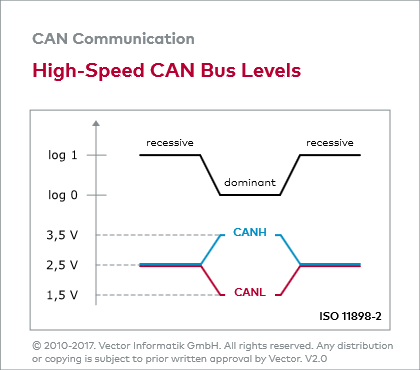
\includegraphics[width=\linewidth]{Figures/can_high_speed_bus_levels.png}
        \par\vspace{0.15cm}
        {\footnotesize Niveles diferenciales CANH/CANL}
    \end{minipage}\hfill
    \begin{minipage}[t]{0.48\textwidth}
        \centering
        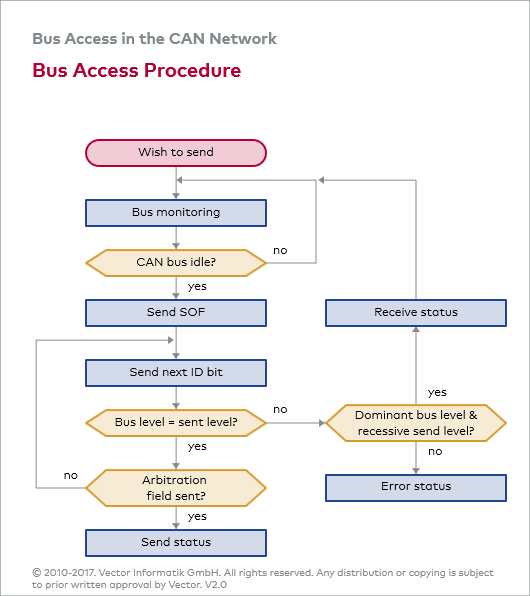
\includegraphics[width=\linewidth]{Figures/can_bus_access_procedure.png}
        \par\vspace{0.15cm}
        {\footnotesize Procedimiento de acceso al bus}
    \end{minipage}
    \caption{Relación entre los niveles diferenciales del bus CAN y el arbitraje por prioridad, adaptado de Vector Informatik \cite{vector2021_can_bus_levels,vector2022_can_bitwise_arbitration}.}
    \label{fig:can-autosense-topologia}
\end{figure}

La transmisión en CAN clásico se realiza sobre dos líneas diferenciales, CANH y CANL, lo que mejora la inmunidad frente al ruido electromagnético presente en el entorno automotriz. Esta propiedad es importante porque el vehículo integra motores, actuadores y otros componentes eléctricos capaces de introducir perturbaciones en la comunicación. El uso de señal diferencial permite mantener la integridad de los mensajes y favorecer una lectura estable desde el firmware del ESP32-S3, incluso cuando el sistema opera con el vehículo en funcionamiento \cite{vector2021_can_bus,vector2021_can_bus_levels}.

Otro rasgo esencial del protocolo es el arbitraje no destructivo por prioridad. Cuando varios nodos intentan transmitir al mismo tiempo, el mensaje con el identificador de menor valor numérico conserva el control del bus, mientras los demás esperan sin corromper la trama ganadora. Este mecanismo evita colisiones y permite que la red mantenga un comportamiento determinista suficiente para aplicaciones de control y diagnóstico. En AutoSense, esta característica resulta útil porque el dispositivo no necesita imponer tráfico propio sobre la red, sino observar y consultar la información permitida respetando la prioridad natural del bus \cite{vector2022_can_bitwise_arbitration}.

\begin{table}[H]
    \centering
    \caption{Elementos básicos del protocolo CAN y su relación con AutoSense.}
    \label{tab:can-autosense-elementos}
    \small
    \begin{tabular}{p{0.18\textwidth}p{0.36\textwidth}p{0.34\textwidth}}
        \toprule
        Elemento & Función & Relevancia en AutoSense \\
        \midrule
        CANH/CANL & Líneas diferenciales del bus & Mejoran la inmunidad al ruido y estabilizan la lectura \\
        ECU & Nodo que transmite y recibe marcos & Origina la información que el sistema consulta \\
        Arbitraje por ID & Resuelve el acceso al medio sin colisiones & Permite coexistir con el tráfico interno del vehículo \\
        Puerto OBD2 & Punto físico de acceso al bus & Conecta el ESP32-S3 sin modificar la red original \\
        Transceptor CAN & Adapta niveles eléctricos entre bus y controlador & Habilita la interfaz de lectura del prototipo \\
        \bottomrule
    \end{tabular}
\end{table}

En AutoSense, el protocolo CAN funciona como la capa de transporte que hace posible la adquisición de datos del vehículo a través del puerto de diagnóstico. El proyecto no busca reorganizar la red ni alterar la lógica interna del automóvil, sino aprovechar la infraestructura existente para obtener información de forma segura y repetible. Por esa razón, el papel del CAN en esta sección es describir el medio de comunicación que soporta la lectura, mientras que la interpretación de parámetros y la consulta de servicios específicos se desarrollan en los apartados posteriores. Esta separación evita repeticiones y deja claro que el protocolo de comunicación cumple una función de soporte dentro de la solución global.

\section{PIDs vehiculares}

Los \textit{Parameter Identifiers} o PIDs constituyen el mecanismo mediante el cual el estándar OBD-II expone magnitudes de diagnóstico normalizadas para consulta externa. Cada PID identifica una variable concreta y define la estructura básica de su respuesta, de modo que el equipo de escaneo pueda interpretar el dato sin depender de la marca o del modelo del vehículo \cite{sae2022_j1978_obdii_scan_tool,sae2025_j1979_diagnostic_test_modes,sae2011_j1979_da}. En AutoSense, esta abstracción es importante porque el sistema no trabaja con una lista abierta de señales, sino con un conjunto controlado de identificadores definidos en los perfiles del proyecto y validados según el vehículo de prueba.

\subsection{Definición y alcance de los PIDs}

En la práctica, AutoSense usa principalmente PIDs de \texttt{Mode 01}, es decir, de lectura de datos en tiempo real. Este modo concentra variables como régimen del motor, velocidad, temperatura, carga y estado de sensores básicos. El anexo digital SAE J1979-DA centraliza la definición de estos identificadores y de otros elementos normalizados, como TIDs, OBDMIDs y tipos de información, lo cual permite que el sistema trate la consulta de forma uniforme aun cuando el vehículo responda con valores distintos o con disponibilidad parcial de parámetros \cite{sae2025_j1979_diagnostic_test_modes,sae2011_j1979_da}.

AutoSense no intenta construir un catálogo exhaustivo de todos los PIDs posibles. La lógica del proyecto parte de dos perfiles reales: \texttt{generic\_obd2}, que agrupa las señales estándar más útiles para operación básica, y \texttt{vw\_passat\_2016}, que añade los identificadores verificados específicamente en el vehículo de referencia. Esta separación mantiene una lectura consistente de acuerdo con el perfil activo.

\subsection{Descubrimiento de PIDs y selección del perfil}

El proceso de descubrimiento comienza con las consultas de soporte del modo 01. AutoSense interroga sucesivamente los bloques \texttt{0100}, \texttt{0120}, \texttt{0140}, \texttt{0160}, \texttt{0180}, \texttt{01A0} y \texttt{01C0}, que funcionan como mapas de disponibilidad de PIDs para el rango estándar. La respuesta de cada bloque permite saber qué identificadores declara la ECU antes de intentar un sondeo más fino. De esta forma, el sistema reduce consultas innecesarias y construye una lista de lectura alineada con el soporte real del vehículo, en lugar de asumir que todos los parámetros están presentes.

Una vez obtenida la disponibilidad básica, el firmware solicita \texttt{Mode 09 PID 02} para recuperar el VIN. Ese dato se utiliza en la aplicación para resolver el perfil de vehículo correspondiente y descargar la configuración correcta desde el backend. En el flujo del proyecto, esta decisión es clave porque el mismo conjunto de respuestas puede interpretarse de manera diferente según la marca, el modelo y el año. Cuando el perfil resuelto es \texttt{vw\_passat\_2016}, el sistema conserva las señales confirmadas para ese vehículo y deja como opcionales aquellas que existen en el estándar, pero que aún no fueron validadas.

Este diseño también explica por qué el archivo de perfil incluye una estructura \texttt{signals[]} con estados distintos de habilitación. El motor de consulta no recorre una lista libre, sino una \textit{allowlist} explícita de PIDs y de fórmulas asociadas. En términos prácticos, el perfil determina qué se consulta, cada cuánto se consulta y si la señal debe quedar activa desde el inicio o permanecer deshabilitada hasta una validación posterior.

\subsection{Conversión de respuesta bruta a unidades de ingeniería}

La utilidad real de un PID no está solo en su identificación, sino en la conversión de la respuesta cruda a una magnitud comprensible. En AutoSense, la decodificación se limita a un conjunto pequeño de transformaciones permitidas, con el fin de mantener el proceso reproducible y fácil de auditar. Para respuestas de un byte, el sistema usa relaciones directas como \texttt{A}, \texttt{A-40} o \texttt{A*100/255}; para respuestas de dos bytes, emplea combinaciones big-endian como \texttt{((A*256)+B)/4}, \texttt{((A*256)+B)/100}, \texttt{((A*256)+B)/1000}, \texttt{A*256+B} y \texttt{(A-128)*100/128}. Esta restricción mantiene la interpretación dentro de las reglas ya verificadas en los perfiles del proyecto.

Con ese criterio, el perfil común utiliza PIDs como \texttt{04} para carga del motor, \texttt{05} para temperatura del refrigerante, \texttt{0B} para presión del múltiple de admisión, \texttt{0C} para revoluciones por minuto, \texttt{0D} para velocidad del vehículo, \texttt{0F} para temperatura del aire de admisión, \texttt{11} para posición del acelerador y \texttt{42} para voltaje de la ECU. Estas señales constituyen la base de lectura en AutoSense porque ofrecen una visión operativa suficiente para registrar estado del motor, demanda del conductor y condiciones generales de funcionamiento. A partir de ellas, el sistema puede construir series de tiempo útiles para visualización y análisis posterior sin entrar en parámetros propietarios complejos.

En el perfil \texttt{vw\_passat\_2016}, AutoSense incorpora además los PIDs \texttt{06} y \texttt{07}, correspondientes a los ajustes de combustible a corto y largo plazo del banco 1, junto con \texttt{1F}, que reporta el tiempo de funcionamiento desde el arranque del motor. El perfil también conserva como opcionales otros PIDs estándar, entre ellos \texttt{10}, \texttt{2F}, \texttt{5C} y \texttt{5E}, que representan masa de aire, nivel de combustible, temperatura del aceite y caudal de combustible. En la configuración actual permanecen desactivados por defecto cuando no existe una verificación directa en el vehículo.

La siguiente tabla resume el conjunto de PIDs utilizado por los perfiles de AutoSense y la función que cumplen dentro de la solución.

\begin{table}[H]
\centering
\scriptsize
\renewcommand{\arraystretch}{1.05}
\setlength{\tabcolsep}{3.5pt}
\begin{tabular}{p{0.09\textwidth}p{0.22\textwidth}p{0.18\textwidth}p{0.39\textwidth}}
\toprule
PID & Magnitud & Perfil & Uso en AutoSense \\
\midrule
04 & Carga del motor & \texttt{generic\_obd2} & Base operativa \\
05 & Temperatura del refrigerante & \texttt{generic\_obd2} & Contexto térmico \\
0B & Presión del múltiple de admisión & \texttt{generic\_obd2} & Lectura de carga \\
0C & Revoluciones por minuto & \texttt{generic\_obd2} & Muestreo principal \\
0D & Velocidad del vehículo & \texttt{generic\_obd2} & Contexto de marcha \\
0F & Temperatura del aire de admisión & \texttt{generic\_obd2} & Apoyo térmico \\
11 & Posición del acelerador & \texttt{generic\_obd2} & Demanda del conductor \\
42 & Voltaje de la ECU & \texttt{generic\_obd2} & Estabilidad eléctrica \\
06 & Ajuste de mezcla a corto plazo B1 & \texttt{vw\_passat\_2016} & Perfil validado \\
07 & Ajuste de mezcla a largo plazo B1 & \texttt{vw\_passat\_2016} & Perfil validado \\
1F & Tiempo de funcionamiento & \texttt{vw\_passat\_2016} & Perfil validado \\
10 / 2F / 5C / 5E & MAF, nivel de combustible, temperatura del aceite y caudal de combustible & \texttt{vw\_passat\_2016} & Opcionales desactivados por defecto \\
\bottomrule
\end{tabular}
\caption{PIDs implementados en los perfiles de AutoSense y su uso funcional.}
\end{table}

En conjunto, esta capa de PIDs convierte el intercambio de bytes con la ECU en una lista de variables legibles y comparables. Esa transformación es la que permite que AutoSense pase de una respuesta técnica de diagnóstico a una interfaz útil para el usuario, manteniendo la lectura dentro del alcance del estándar y del vehículo validado.

\section{Microcontrolador ESP32}
\label{sec:microcontrolador-esp32}

El ESP32-S3 constituye el núcleo embebido de AutoSense. En la arquitectura del prototipo, su función no se limita a actuar como interfaz de comunicación, sino que concentra la adquisición de datos del vehículo, la aplicación de la política de solo lectura, el manejo del perfil activo y la redistribución de la información hacia las capas de presentación y almacenamiento. Esta organización permite que la solución permanezca compacta, con una secuencia de operación reproducible entre arranques y con un único punto de control para la lógica embebida.

\subsection{Arquitectura del microcontrolador}

El ESP32-S3 opera como nodo central porque articula tres tareas que en AutoSense no conviene separar en controladores distintos: leer el bus del vehículo, validar qué solicitudes están permitidas y entregar el resultado a los módulos que lo necesitan. Espressif documenta para esta familia soporte de Bluetooth Low Energy y de USB OTG/USB CDC, capacidades que en el prototipo se aprovechan para mover datos entre el microcontrolador, la aplicación móvil y el entorno de supervisión local \cite{espressif2026_esp32s3_get_started,espressif2026_esp32s3_usb_otg_console}. La explicación detallada de esos enlaces se reserva para la sección de comunicaciones; aquí interesa el papel del ESP32-S3 como coordinador del flujo de información.

En AutoSense, esa coordinación evita que la lógica quede repartida entre el firmware, la aplicación y el almacenamiento. El microcontrolador recibe el resultado de la consulta vehicular, lo convierte en estructuras internas de trabajo y mantiene la continuidad del estado entre ciclos de muestreo. De ese modo, el prototipo no depende de una lectura aislada, sino de una ejecución ordenada que conserva el contexto del vehículo activo y de las señales habilitadas.

\subsection{Funciones del ESP32-S3 en AutoSense}

Durante el arranque, el firmware sigue una secuencia fija. Primero inicializa la consola, los periféricos básicos y el transceptor CAN; luego carga la configuración local desde \texttt{data/config.ini}; después intenta recuperar \texttt{/active\_profile.json} cuando ya existe un perfil aplicado por la aplicación; y finalmente arranca los servicios de consulta, el dashboard, el registro histórico y el enlace BLE. Esa secuencia es relevante porque deja al sistema en un estado conocido antes de comenzar el sondeo de datos del vehículo.

El archivo \texttt{active\_profile.json} cumple una función central en esa etapa. Allí se conserva el perfil vehicular que define qué PIDs se consultan, con qué fórmulas se decodifican y qué señales se consideran válidas para el contexto actual. Así, el ESP32-S3 no improvisa la lectura ni trabaja con una lista abierta de parámetros; por el contrario, aplica la configuración que la aplicación resolvió a partir del VIN y del vehículo validado. Esta decisión mantiene la coherencia entre el perfil seleccionado, el plan de muestreo y la información que luego ve el usuario.

Otra función clave del microcontrolador es el control de la política de solo lectura. Antes de emitir solicitudes al vehículo, el firmware pasa por un guardián que bloquea operaciones de borrado, control o reprogramación. Con ello, AutoSense se limita a observar y registrar, sin intervenir la ECU ni modificar la condición del automóvil durante las pruebas. Este criterio también simplifica la validación, porque el estado del vehículo no cambia por efecto del propio prototipo y las mediciones pueden repetirse bajo condiciones más estables.

\subsection{Integración con almacenamiento y salida de datos}

Además de consultar el vehículo, el ESP32-S3 organiza la persistencia local y la salida de información. El almacenamiento sobre LittleFS se usa para conservar la configuración operativa y el perfil activo, mientras que el historial se mantiene en una representación compacta dentro de la flash interna del dispositivo. Esta separación evita mezclar datos de control con datos de telemetría y hace posible reiniciar el sistema sin perder la referencia de trabajo más reciente.

En la salida de datos, AutoSense emplea dos canales complementarios. El primero es el dashboard por USB-CDC, pensado para supervisión local y depuración durante las pruebas. El segundo es el enlace BLE hacia la aplicación móvil, donde el usuario ve las lecturas ya interpretadas y el estado general del vehículo. La discusión detallada de esos canales se presenta en la sección de comunicaciones; en este punto basta señalar que el ESP32-S3 actúa como puente entre el vehículo y la capa de presentación, traduciendo bytes de diagnóstico en información utilizable por el resto del sistema.

En conjunto, el microcontrolador no es solo un componente de control, sino la pieza que hace posible la continuidad del flujo de AutoSense. Su valor dentro del prototipo radica en que concentra adquisición, validación, persistencia y distribución de datos en un único nodo embebido, lo que reduce la complejidad de integración y mantiene alineadas las decisiones de firmware con el perfil vehicular activo.

\section{Internet de las Cosas}
\label{sec:iot}

La Internet de las Cosas constituye el marco conceptual que permite tratar al vehículo como una fuente continua de datos y no solo como un sistema que entrega información bajo consulta puntual. En el contexto automotriz, esta perspectiva integra sensores embarcados, procesamiento en el borde y servicios remotos para capturar, organizar y explotar datos de operación, diagnóstico y comportamiento del conductor. Diversos trabajos han mostrado que esta aproximación facilita la supervisión remota del vehículo, la detección oportuna de anomalías y la construcción de historiales útiles para mantenimiento y administración \cite{shafi2018_vehicle_remote_health,camposferreira2023_vehicle_driver_monitoring,singh2021_obdii_iot,dabarera2022_iot_vehicle_management,zhang2020_iov_edge}.

\subsection{Internet de las Cosas en vehículos conectados}

En vehículos conectados, la IoT no se limita a enlazar un dispositivo con una aplicación móvil. Su aporte principal consiste en distribuir funciones entre la captura local, la primera normalización de datos y la disponibilidad remota de la información. La literatura reciente sobre Internet de los Vehículos y computación en el borde destaca que esta separación mejora la respuesta del sistema y reduce la dependencia de un servidor central para tareas que pueden resolverse cerca de la fuente de datos \cite{zhang2020_iov_edge}. En AutoSense, ese criterio se materializa en un flujo donde el vehículo produce los datos, el ESP32-S3 los adquiere y filtra, y la capa remota conserva únicamente la información que resulta útil para el usuario y para el seguimiento del estado del vehículo.

Desde esa perspectiva, AutoSense se comporta como un sistema conectado de monitoreo vehicular más que como un simple lector de diagnóstico. La propuesta no busca enviar todo el tráfico bruto a la nube, sino seleccionar señales relevantes, mantener un perfil vehicular activo y presentar al usuario una visión organizada del estado del automóvil. Este enfoque coincide con soluciones IoT de monitoreo y telemetría vehicular que combinan lectura embarcada, visualización remota y apoyo a la toma de decisiones \cite{shafi2018_vehicle_remote_health,camposferreira2023_vehicle_driver_monitoring}.

\subsection{AutoSense como arquitectura borde-nube}

AutoSense se organiza como una arquitectura borde-nube. En el borde se ubica el ESP32-S3, que concentra la adquisición inicial, la aplicación de la política de solo lectura y la preparación de los datos para su consumo por la aplicación. En la capa intermedia está la app móvil, que funciona como interfaz de visualización, selección de perfil y supervisión del estado del dispositivo. Finalmente, la nube ofrece persistencia, sincronización y trazabilidad para perfiles, estado de conexión e historial asociado al usuario. Esta división permite que el sistema conserve la respuesta rápida local y, al mismo tiempo, mantenga disponibilidad remota de la información que debe persistir entre sesiones.

La relación entre estas capas puede representarse de forma conceptual como sigue:

\begin{figure}[H]
    \centering
    \begingroup
    \shorthandoff{>}
    \begin{tikzpicture}[
        font=\small,
        node distance=8mm,
        >=Latex,
        veh/.style={draw=gray!70!black, rounded corners=5pt, fill=gray!10, line width=0.9pt, align=center, text width=4.8cm, minimum height=1.0cm, inner sep=5pt},
        core/.style={draw=blue!70!black, rounded corners=5pt, fill=blue!11, line width=0.9pt, align=center, text width=4.8cm, minimum height=1.05cm, inner sep=5pt},
        app/.style={draw=green!60!black, rounded corners=5pt, fill=green!11, line width=0.9pt, align=center, text width=4.8cm, minimum height=1.05cm, inner sep=5pt},
        cloud/.style={draw=teal!70!black, rounded corners=5pt, fill=teal!11, line width=0.9pt, align=center, text width=4.8cm, minimum height=1.05cm, inner sep=5pt},
        link/.style={draw=black!75, line width=1pt, -{Latex[length=3mm,width=2mm]}}
    ]
        \node[veh] (veh) {Vehículo\\\scriptsize Fuente de datos OBD-II / CAN};
        \node[core, below=of veh] (esp32) {ESP32-S3\\\scriptsize Adquisición local y política de lectura};
        \node[app, below=of esp32] (appnode) {Aplicación móvil\\\scriptsize BLE, perfil activo y visualización};
        \node[cloud, below=of appnode] (cloud) {Firebase / nube\\\scriptsize Persistencia y sincronización remota};

        \draw[link] (veh) -- node[right, xshift=4pt, font=\scriptsize] {OBD-II / CAN} (esp32);
        \draw[link, violet!80!black] (esp32) -- node[right, xshift=4pt, font=\scriptsize] {BLE} (appnode);
        \draw[link, teal!70!black] (appnode) -- node[right, xshift=4pt, font=\scriptsize] {Wi-Fi} (cloud);
    \end{tikzpicture}
    \endgroup
    \caption{Arquitectura vertical de la IoT de AutoSense.}
\end{figure}

La función del ESP32-S3 dentro de esta arquitectura es central porque actúa como nodo de borde: recibe la información del vehículo, aplica las validaciones básicas del firmware y entrega solo aquello que debe circular hacia la aplicación. La capa móvil, por su parte, no se limita a mostrar valores; también coordina la identificación del vehículo, el manejo del perfil activo y la experiencia del usuario, de manera que la nube reciba datos ya contextualizados y no lecturas aisladas.

\subsection{Sincronización y supervisión remota}

La dimensión IoT de AutoSense se consolida cuando la información deja de ser estrictamente local y pasa a formar parte de un ecosistema sincronizado. En el proyecto, Firebase cumple ese papel de soporte remoto: ayuda a resolver perfiles, conservar estado de usuario, registrar aplicación de perfiles y mantener consistencia entre sesiones. Esa estrategia permite que el sistema no dependa de una sola ejecución del firmware para conocer el contexto del vehículo, sino que reutilice datos ya validados para acelerar la interacción futura con la plataforma.

La supervisión remota también es importante porque convierte el monitoreo en una actividad continua y no solo en una lectura ocasional. El usuario puede retomar el estado del vehículo, revisar la información sincronizada y visualizar el historial sin reinstalar ni reconfigurar todo el sistema. En otras palabras, AutoSense usa la IoT para enlazar adquisición local, visualización inmediata y persistencia remota dentro de una misma cadena de trabajo. Ese diseño es coherente con propuestas de gestión vehicular y diagnóstico remoto basadas en OBD2, donde el valor del sistema está en integrar telemetría, conectividad y trazabilidad de la información \cite{singh2021_obdii_iot,dabarera2022_iot_vehicle_management}.

La siguiente sección desarrolla la comunicación Bluetooth, Wi-Fi y USB, que es el mecanismo concreto mediante el cual esta arquitectura de borde y nube intercambia datos entre el ESP32-S3, la aplicación y los servicios auxiliares.

\section{Comunicación Bluetooth, Wi-Fi y USB}
\label{sec:comunicacion}

La comunicación de AutoSense reúne los canales que permiten mover la información desde el ESP32-S3 hacia la aplicación móvil y, desde allí, hacia los servicios remotos. En esta sección no se retoma el detalle de OBD2 ni del bus CAN, porque esa parte ya fue desarrollada en los apartados anteriores; aquí interesa el medio de transporte de los datos dentro de la arquitectura del prototipo. En el caso del ESP32-S3, Espressif documenta el soporte de Bluetooth Low Energy y de USB OTG/USB-CDC para esta familia, capacidades que el proyecto aprovecha para separar la supervisión local del intercambio inalámbrico con el teléfono \cite{espressif2026_esp32s3_get_started,espressif2026_esp32s3_ble_overview,espressif2026_esp32s3_usb_otg_console}.

\subsection{Bluetooth Low Energy}

Bluetooth Low Energy constituye el canal principal de enlace entre el ESP32-S3 y la aplicación móvil de AutoSense. En el repositorio, el dispositivo anuncia el nombre \texttt{AutoSense OBD2}, expone un servicio GATT propio y utiliza dos características diferenciadas: una para recibir comandos desde la app y otra para notificar respuestas y telemetría. Esa separación facilita que la app actúe como cliente y que el firmware permanezca como periférico, manteniendo un flujo simple de descubrimiento, conexión y lectura de datos.

El intercambio por BLE no se limita a enviar valores en vivo. La aplicación también utiliza este canal para solicitar información del dispositivo, leer el estado del perfil activo, aplicar perfiles de vehículo y activar o detener el flujo de telemetría. En consecuencia, BLE funciona como la interfaz operativa del usuario con el sistema embebido: desde allí se desencadena la sesión de diagnóstico, se reciben notificaciones periódicas con las señales decodificadas y se actualiza la vista móvil sin necesidad de cables. Esa elección es coherente con la implementación del proyecto, donde la comunicación con el celular se resuelve mediante GATT y notificaciones, mientras la carga de trabajo pesada permanece en el firmware del ESP32-S3.

\subsection{USB-CDC}

USB-CDC cumple una función distinta: no enlaza al teléfono, sino que habilita la consola local y el dashboard del firmware. Durante el arranque, el ESP32-S3 publica un estado de ejecución que incluye el transporte \texttt{USB-CDC+BLE}, y la salida por USB se usa para observar diagnósticos, revisar el progreso de la conexión y depurar el comportamiento del sistema sin depender de la app móvil. Esta ruta resulta útil en desarrollo y validación porque entrega retroalimentación inmediata sobre el estado del vehículo, el perfil activo y la operación del firmware.

En AutoSense, por tanto, USB-CDC debe entenderse como un canal de supervisión local, no como el medio de emparejamiento con el usuario final. Su valor práctico está en que ofrece una vista directa del prototipo mientras BLE mantiene la sesión de intercambio con la aplicación. Esta separación reduce la interferencia entre monitoreo técnico y experiencia de uso, y permite que la depuración del firmware se realice sin alterar la lógica de comunicación pensada para el teléfono.

\subsection{Wi-Fi y sincronización remota}

Wi-Fi se trata en AutoSense como el medio de conectividad de la aplicación hacia los servicios remotos, no como un enlace activo del ESP32-S3 con la ECU o con el módulo de adquisición. En la arquitectura del proyecto, la sincronización con Firebase ocurre desde la capa móvil, donde se conservan perfiles, estado de usuario e información asociada a la sesión. Con ello, el sistema mantiene una separación clara: el dispositivo embebido adquiere y transmite por BLE, mientras la aplicación gestiona la persistencia y la sincronización cuando existe acceso a red.

Esta decisión evita duplicar funciones de comunicación dentro del firmware y permite que el prototipo conserve un comportamiento simple en el borde. En términos prácticos, Wi-Fi aparece como el soporte de la nube y no como la ruta interna de diagnóstico; de esa manera, la información puede respaldarse, recuperarse o actualizarse desde el ecosistema móvil sin modificar el flujo principal de lectura del vehículo. La próxima sección desarrolla la aplicación móvil, que es donde estos canales se integran en una interfaz de uso cotidiano.

\begin{figure}[H]
    \centering
    \begingroup
    \shorthandoff{>}
    \begin{tikzpicture}[
        font=\small,
        node distance=12mm and 28mm,
        >=Latex,
        data/.style={draw=gray!65!black, rounded corners=4pt, fill=gray!8, line width=0.8pt, align=center, text width=3.0cm, minimum height=1.2cm, inner sep=5pt},
        core/.style={draw=blue!70!black, rounded corners=4pt, fill=blue!10, line width=0.9pt, align=center, text width=3.2cm, minimum height=1.3cm, inner sep=6pt},
        ble/.style={draw=violet!70!black, rounded corners=4pt, fill=violet!12, line width=0.9pt, align=center, text width=3.15cm, minimum height=1.25cm, inner sep=5pt},
        app/.style={draw=green!60!black, rounded corners=4pt, fill=green!12, line width=0.9pt, align=center, text width=3.1cm, minimum height=1.25cm, inner sep=5pt},
        cloud/.style={draw=teal!70!black, rounded corners=4pt, fill=teal!10, line width=0.9pt, align=center, text width=3.05cm, minimum height=1.25cm, inner sep=5pt},
        usb/.style={draw=orange!80!black, rounded corners=4pt, fill=orange!14, line width=0.9pt, align=center, text width=2.9cm, minimum height=1.15cm, inner sep=5pt},
        console/.style={draw=orange!60!black, rounded corners=4pt, fill=orange!8, line width=0.8pt, align=center, text width=3.0cm, minimum height=1.15cm, inner sep=5pt},
        link/.style={draw=black!75, line width=1pt, -{Latex[length=3mm,width=2mm]}}
    ]
        \node[data] (vehicle) {Vehículo\\OBD-II / CAN};
        \node[core, below=of vehicle] (esp32) {ESP32-S3\\\scriptsize Firmware AutoSense\\\scriptsize LittleFS + políticas de lectura};

        \node[ble, below=of esp32] (ble) {Bluetooth Low Energy\\\scriptsize Servicio GATT\\\scriptsize RX / TX};
        \node[app, below=of ble] (app) {Aplicación móvil\\\scriptsize react-native-ble-plx\\\scriptsize Sesión y telemetría};
        \node[cloud, below=of app] (cloud) {Wi-Fi / Internet\\\scriptsize Firebase\\\scriptsize Sincronización remota};

        \node[usb, right=of esp32] (usb) {USB-CDC\\\scriptsize Dashboard local};
        \node[console, below=of usb] (console) {Monitor serial\\\scriptsize Depuración y estado};

        \draw[link] (vehicle) -- node[right, xshift=4pt, font=\scriptsize] {Lectura vehicular} (esp32);
        \draw[link, violet!80!black] (esp32) -- node[right, xshift=4pt, font=\scriptsize] {BLE} (ble);
        \draw[link, green!60!black] (ble) -- node[right, xshift=4pt, font=\scriptsize] {Comandos / telemetría} (app);
        \draw[link, teal!70!black] (app) -- node[right, xshift=4pt, font=\scriptsize] {Wi-Fi} (cloud);
        \draw[link, orange!85!black] (esp32) -- node[above, font=\scriptsize] {USB-CDC} (usb);
        \draw[link, orange!70!black] (usb) -- node[right, xshift=4pt, font=\scriptsize] {Dashboard} (console);
    \end{tikzpicture}
    \endgroup
    \caption{Diagrama vertical de los canales de comunicación de AutoSense.}
\end{figure}

\noindent En síntesis, BLE sostiene la interacción principal con el usuario, USB-CDC cubre la supervisión técnica local y Wi-Fi respalda la sincronización remota desde la aplicación. Esa división mantiene el prototipo simple, consistente y alineado con el flujo real implementado en el repositorio.

\section{Aplicaciones móviles}

\label{sec:aplicaciones-moviles}

La aplicación móvil de AutoSense constituye la capa visible de interacción del sistema. Desde ella se administra el acceso, se selecciona el vehículo activo, se supervisa el estado de conexión y se consulta la telemetría que proviene del ESP32-S3. Su diseño no intenta duplicar la lógica embebida, sino presentar en una interfaz portátil la información que ya fue adquirida y validada en el borde. Para ello, el proyecto se apoya en React Native, Expo Router y Firebase, con una organización que permite mantener un mismo flujo funcional en Android e iOS.

\subsection{Arquitectura interna de la aplicación}

La base de la aplicación se organiza mediante rutas y contexto de sesión. El flujo está dividido en dos grupos principales: \texttt{Auth}, que concentra el ingreso y el registro, y \texttt{App}, que agrupa las pantallas de uso cotidiano una vez autenticado el usuario. Esa separación reduce el acoplamiento entre el acceso y la operación del vehículo, y permite que la navegación responda al estado real de la cuenta. En la raíz, \texttt{SessionProvider} escucha el estado de Firebase Auth, hidrata el perfil desde Firestore y conserva la sesión en SecureStore para evitar que el usuario deba autenticarse en cada apertura. A partir de ese contexto, \texttt{AuthLayout} mantiene al usuario fuera del área operativa cuando no existe sesión activa, mientras que \texttt{AppLayout} entrega directamente las pestañas principales cuando la sesión ya está resuelta.

Sobre esa base, la app utiliza una navegación por pestañas con tres destinos principales: \texttt{Inicio}, \texttt{Tiempo real} y \texttt{Perfil}. Esta decisión simplifica el uso diario porque concentra en pocos accesos las tareas más frecuentes: revisar el estado general del vehículo, enlazar el dispositivo OBD2 por BLE y administrar los datos de la cuenta. El resto de pantallas se despliega como rutas secundarias, de modo que la experiencia principal permanece limpia y con una jerarquía clara.

\begin{figure}[H]
    \centering
    \begingroup
    \shorthandoff{>}
    \begin{tikzpicture}[
        font=\small,
        node distance=7mm,
        >=Latex,
        accessbox/.style={draw=blue!70!black, rounded corners=5pt, fill=blue!9, line width=0.9pt, align=center, text width=11.3cm, minimum height=1.2cm, inner sep=6pt},
        session/.style={draw=violet!75!black, rounded corners=5pt, fill=violet!12, line width=0.9pt, align=center, text width=11.3cm, minimum height=1.25cm, inner sep=6pt},
        nav/.style={draw=green!60!black, rounded corners=5pt, fill=green!11, line width=0.9pt, align=center, text width=11.3cm, minimum height=1.25cm, inner sep=6pt},
        screens/.style={draw=orange!80!black, rounded corners=5pt, fill=orange!12, line width=0.9pt, align=center, text width=11.3cm, minimum height=1.4cm, inner sep=6pt},
        integrations/.style={draw=teal!70!black, rounded corners=5pt, fill=teal!11, line width=0.9pt, align=center, text width=11.3cm, minimum height=1.45cm, inner sep=6pt},
        link/.style={draw=black!70, line width=1pt, -{Latex[length=3mm,width=2mm]}}
    ]
        \node[accessbox] (access) {Acceso y registro\\\scriptsize Inicio de sesión con correo y Google, recuperación de cuenta y registro guiado en tres pasos};
        \node[session, below=of access] (sessionnode) {Gestión de sesión\\\scriptsize \texttt{SessionProvider}, SecureStore y Firebase Auth para mantener el estado del usuario};
        \node[nav, below=of sessionnode] (navigation) {Navegación principal\\\scriptsize \texttt{Auth} / \texttt{App} y pestañas \texttt{Inicio}, \texttt{Tiempo real} y \texttt{Perfil}};
        \node[screens, below=of navigation] (screens) {Pantallas operativas\\\scriptsize Inicio con tablero, eficiencia, viajes y alertas; emparejamiento BLE; vista en vivo; perfil, vehículo, datos personales y ajustes};
        \node[integrations, below=of screens] (integrations) {Integraciones de la app\\\scriptsize BLE nativo con \texttt{react-native-ble-plx} y sincronización con Firebase Auth, Firestore, Functions y Storage};

        \draw[link] (access) -- (sessionnode);
        \draw[link] (sessionnode) -- (navigation);
        \draw[link] (navigation) -- (screens);
        \draw[link] (screens) -- (integrations);
    \end{tikzpicture}
    \endgroup
    \caption{Flujo vertical de la aplicación móvil de AutoSense.}
    \label{fig:autosense-mobile-architecture}
\end{figure}

La figura resume el recorrido interno de la aplicación: primero se resuelve el acceso, luego se consolida la sesión, después se expone la navegación principal y, por último, se conectan los servicios que sostienen la operación del sistema. Esa secuencia evita que la interfaz móvil sea solo una colección de pantallas sueltas y la convierte en una capa coherente de control sobre la información del vehículo.

\subsection{Pantallas y flujo de uso}

La pantalla inicial de AutoSense actúa como puerta de entrada. Allí el usuario puede iniciar sesión con correo y contraseña o con Google, además de recuperar su cuenta si olvidó la clave. El flujo de registro está dividido en tres pasos: primero se captura el correo, luego se completan los datos básicos y finalmente se define la contraseña. Esa división reduce la fricción en el alta de usuarios y mantiene el proceso de autenticación alineado con la estructura interna de Firebase.

Una vez autenticado, el apartado \texttt{Inicio} funciona como tablero principal. Desde allí se presenta el vehículo activo, el nivel de combustible estimado, la eficiencia, el estilo de conducción, el viaje actual y las alertas prioritarias. Cuando el sistema todavía no cuenta con un dispositivo enlazado o con telemetría histórica suficiente, la pantalla muestra un llamado a conectar el AutoSense ESP32 y pasar a \texttt{Tiempo real}. Esta lógica evita que la interfaz prometa datos que todavía no existen y deja claro qué información proviene de una lectura real y cuál aún depende de la conexión del prototipo.

El módulo de \texttt{Tiempo real} está dividido en dos momentos. El primero es el emparejamiento, donde la app busca el dispositivo \texttt{AutoSense OBD2} por Bluetooth, establece la conexión y resuelve el perfil vehicular activo. En esa etapa se verifica el VIN cuando está disponible, se aplica el perfil correcto y se prepara el canal de telemetría. El segundo momento es la vista en vivo, donde aparecen métricas como velocidad, RPM, temperatura del motor, consumo estimado, carga, voltaje, posición del acelerador y temperatura de admisión, junto con un resumen del estado del sistema. Además, la sesión en vivo sincroniza el seguimiento del viaje y actualiza el tablero remoto, de modo que la app no solo visualiza datos sino que también los incorpora al historial del usuario.

El apartado \texttt{Perfil} organiza la administración de la cuenta y del vehículo. Desde allí se puede revisar el vehículo actual, editar datos personales, cambiar correo, modificar contraseña, ajustar preferencias de unidades, alertas y privacidad, y cerrar sesión. La pantalla de vehículo permite cambiar el perfil base del automóvil y el estado de enlace, mientras que las pantallas de detalles separan la información personal del control de seguridad. Esta estructura mantiene el perfil de usuario como una entidad central de la experiencia y evita que la configuración quede repartida entre pantallas inconexas.

El resto de la navegación complementa esa lógica principal. Las vistas de eficiencia, viajes y alertas amplían la información del tablero con trayectos previos, análisis de conducción y avisos puntuales. En conjunto, la aplicación no se limita a mostrar números; organiza la relación entre usuario, vehículo y sesión activa para que el seguimiento del automóvil sea continuo y fácil de interpretar.

\subsection{Compatibilidad y despliegue}

La aplicación se desarrolla con Expo SDK 56 y React Native 0.85.3, por lo que su compatibilidad se define por la plataforma y por la capacidad del dispositivo, no por un modelo específico de teléfono. De acuerdo con la documentación oficial de Expo, el SDK vigente soporta Android 7+ e iOS 16.4+ \cite{expo2026_sdk_support}. En la práctica, esto significa que AutoSense puede desplegarse en terminales que ejecuten esas versiones o superiores y que además dispongan de Bluetooth Low Energy para sostener el enlace con el ESP32-S3.

El uso de BLE nativo obliga a trabajar con un \textit{development build} y no con Expo Go. La propia documentación de Expo indica que los \textit{development builds} incluyen \texttt{expo-dev-client} y permiten usar bibliotecas nativas que no están disponibles en Expo Go \cite{expo2026_development_build}. Esta condición no es un detalle de implementación menor: es la que permite que AutoSense use \texttt{react-native-ble-plx} para descubrir, conectar y notificar telemetría sin renunciar al resto del ecosistema de Expo.

En términos de operación, la compatibilidad se expresa mejor como un conjunto de requisitos mínimos: sistema operativo soportado, Bluetooth Low Energy disponible y acceso a los permisos que el sistema pide para conectar con el dispositivo. Bajo esas condiciones, la app mantiene una experiencia estable en Android y iOS, y la misma base de código cubre ambas plataformas sin obligar a mantener dos implementaciones separadas.

Con esta base, la siguiente sección desarrolla la inteligencia artificial, que aprovecha la telemetría ya capturada por la aplicación para construir análisis de comportamiento y apoyo al diagnóstico.

\section{Inteligencia artificial}

\label{sec:inteligencia-artificial}

La inteligencia artificial de AutoSense se ejecuta en el borde y se apoya en los datos compactos que ya produce el firmware, no en una capa externa que reinterprete la señal desde cero. Esa decisión sigue la tendencia descrita por la literatura reciente sobre inteligencia móvil en el Internet de los Vehículos y telemática de tiempo real, donde el valor no está únicamente en captar datos, sino en analizarlos cerca de la fuente para reducir latencia y conservar contexto \cite{zhang2020_iov_edge,selvaraj2023_advanced_telematics,kalalas2025_ai_driven_monitoring}. En AutoSense, la IA no pretende emitir un diagnóstico mecánico definitivo, sino detectar desviaciones, conservar una línea base por vehículo y aportar contexto explicable al usuario mediante indicadores como severidad, área probable y señales más alejadas de lo normal \cite{michailidis2025_obdii_review,tormos2025_explainable_ai,mahale2025_review_predictive_maintenance}.

\subsection{Arquitectura de la IA local}

El módulo de IA de AutoSense consume el mismo \texttt{ObdCompactSample} que ya alimenta el logger binario y la telemetría BLE. Esto evita enviar nuevas solicitudes OBD al vehículo y mantiene el costo computacional bajo, porque la inferencia se ejecuta sobre una muestra ya depurada. En la práctica, el firmware llama al detector cada \texttt{anomaly.interval\_seconds} segundos, que por defecto es 10 s, y solo si existe al menos una muestra válida. Si no hay datos suficientes o la función está deshabilitada, el detector devuelve un resultado vacío y no fuerza decisiones artificiales.

\begin{figure}[H]
    \centering
    \begingroup
    \shorthandoff{>}
    \begin{tikzpicture}[
        font=\small,
        node distance=7mm,
        >=Latex,
        sample/.style={draw=gray!70!black, rounded corners=5pt, fill=gray!10, line width=0.9pt, align=center, text width=11.2cm, minimum height=1.05cm, inner sep=6pt},
        stats/.style={draw=blue!70!black, rounded corners=5pt, fill=blue!10, line width=0.9pt, align=center, text width=11.2cm, minimum height=1.15cm, inner sep=6pt},
        zscore/.style={draw=violet!75!black, rounded corners=5pt, fill=violet!12, line width=0.9pt, align=center, text width=11.2cm, minimum height=1.15cm, inner sep=6pt},
        forest/.style={draw=green!60!black, rounded corners=5pt, fill=green!11, line width=0.9pt, align=center, text width=11.2cm, minimum height=1.15cm, inner sep=6pt},
        output/.style={draw=orange!80!black, rounded corners=5pt, fill=orange!12, line width=0.9pt, align=center, text width=11.2cm, minimum height=1.2cm, inner sep=6pt},
        link/.style={draw=black!70, line width=1pt, -{Latex[length=3mm,width=2mm]}}
    ]
        \node[sample] (sample) {Muestra compacta\\\scriptsize RPM, velocidad, temperatura, carga, throttle, combustible, MAF, MAP, voltaje, admisión y spark advance};
        \node[stats, below=of sample] (statsnode) {Baseline por vehículo y contexto\\\scriptsize Welford global + Welford por contexto; la identidad del perfil reinicia el modelo cuando cambia el vehículo};
        \node[zscore, below=of statsnode] (znode) {Z-score por señal\\\scriptsize desviación respecto de la media local con piso mínimo de desviación estándar};
        \node[forest, below=of znode] (forestnode) {Isolation Forest pequeño\\\scriptsize 16 árboles, sample size 64, profundidad máxima 6, inferencia sin memoria dinámica};
        \node[output, below=of forestnode] (outputnode) {Salida interpretada\\\scriptsize score, severidad, areaMask, topSignals, baselineReady y modelReady};

        \draw[link] (sample) -- (statsnode);
        \draw[link] (statsnode) -- (znode);
        \draw[link] (znode) -- (forestnode);
        \draw[link] (forestnode) -- (outputnode);
    \end{tikzpicture}
    \endgroup
    \caption{Pipeline local de inteligencia artificial de AutoSense.}
    \label{fig:autosense-ai-pipeline}
\end{figure}

La figura resume el recorrido de la IA local: primero se consolida la muestra, luego se construye la referencia estadística, después se estima cuán lejos está la señal de esa referencia y, finalmente, se calcula un score interpretado por el sistema. Esta secuencia es importante porque separa la observación estadística del juicio final, lo que permite que AutoSense funcione con un modelo ligero pero todavía explicable.

\subsection{Baseline estadístico y Z-score}

La primera capa del detector es estadística. El firmware mantiene una línea base con estadísticos acumulados por vehículo y por contexto de conducción mediante el método de Welford, que permite actualizar media y varianza sin guardar todas las muestras históricas. El baseline se divide en una referencia global y referencias por contexto: \texttt{IDLE}, \texttt{CRUISING}, \texttt{ACCELERATING}, \texttt{DECELERATING} y \texttt{UNKNOWN}. Cuando existe suficiente historial contextual, el detector usa el contexto específico; si todavía no hay suficientes muestras, recurre al baseline global. Esa lógica evita que una condición de manejo poco frecuente sesgue toda la referencia del vehículo.

El estado \texttt{baselineReady} no se activa con cualquier dato aislado. En el firmware, la condición mínima exige suficientes muestras válidas por señal y, por defecto, al menos 300 observaciones para considerar estable la referencia. Mientras ese umbral no se cumple, el detector conserva el comportamiento de aprendizaje y limita la interpretación de anomalías. Además, el perfil activo forma parte de la identidad del modelo; si cambia el vehículo o cambia el hash del perfil, la línea base se reinicia para no mezclar comportamientos incompatibles.

La puntuación Z-score se calcula señal por señal como la distancia respecto de la media local normalizada por su desviación estándar. En AutoSense se usa un piso mínimo de desviación por señal para evitar que una variable casi constante produzca falsos positivos. En términos conceptuales, el cálculo puede expresarse así:

\begin{equation}
z_i = \frac{|x_i - \mu_i|}{\max(\sigma_i,\sigma_{\min,i})}
\end{equation}

\begin{equation}
score_z = \mathrm{clamp}\left(\mathrm{rms}(z_i)\cdot 12.5,\ 0,\ 100\right)
\end{equation}

El resultado no se interpreta como una avería concreta, sino como una medida de separación respecto del comportamiento normal del vehículo. Por eso el sistema conserva tres salidas adicionales: las señales con mayor desviación, el área probable asociada a esas señales y la condición de si el baseline ya es suficientemente confiable para seguir aprendiendo.

\subsection{Isolation Forest compacto}

La segunda capa del detector es un \textit{Isolation Forest} pequeño diseñado para ejecutarse en el ESP32-S3 sin memoria dinámica durante la inferencia. El modelo usa 16 árboles, un tamaño de muestra de 64, una ventana circular de 128 muestras y una profundidad máxima de 6 niveles. Esa configuración busca equilibrar costo computacional y sensibilidad, porque el objetivo no es construir un modelo pesado de laboratorio, sino una detección robusta que pueda mantenerse activa mientras el vehículo circula.

El entrenamiento local ocurre solo cuando el contexto es estable. El firmware usa muestras de \texttt{IDLE} o \texttt{CRUISING} para alimentar el bosque y evita aprender a partir de escenarios claramente anómalos o demasiado inestables. Si el bosque aún no está listo, el score final depende exclusivamente del Z-score. Cuando ya existe modelo, el detector combina ambas señales con los pesos configurados en el firmware; por defecto, 70\% para Z-score y 30\% para Isolation Forest. Esta combinación favorece la interpretación estadística de la línea base, pero deja al bosque la tarea de reforzar patrones que no siempre se expresan como una desviación puntual de una sola señal.

\begin{table}[H]
    \centering
    \caption{Parámetros por defecto del detector de anomalías local.}
    \label{tab:ai-anomaly-defaults}
    \renewcommand{\arraystretch}{1.08}
    \setlength{\tabcolsep}{4pt}
    \begin{tabular}{p{0.26\textwidth}p{0.18\textwidth}p{0.48\textwidth}}
    \toprule
    Parámetro & Valor por defecto & Función \\
    \midrule
    Inferencia local & 10 s & Frecuencia de inferencia local. \\
    Baseline mínimo & 300 muestras & Cantidad mínima de muestras para estabilizar el baseline. \\
    Persistencia & 300 s & Intervalo de persistencia del baseline y del modelo. \\
    Ponderación Z & 70\% & Peso del componente estadístico. \\
    Ponderación IF & 30\% & Peso del componente de bosque de aislamiento. \\
    Bosque pequeño & 16 árboles / 64 muestras / profundidad 6 & Configuración compacta para inferencia en el borde. \\
    \bottomrule
    \end{tabular}
\end{table}

El bosque y la línea base se persisten en almacenamiento local para no empezar desde cero en cada reinicio. El baseline se guarda en la partición de preferencias del firmware y el modelo del bosque se exporta como un archivo binario compacto en LittleFS. Ambos artefactos están ligados a la identidad del vehículo y del perfil activo, de modo que AutoSense puede recuperar el estado anterior si no cambió el contexto de trabajo.

\subsection{Salida interpretada y clasificación de ruta}

La salida del detector no se limita a un número. El firmware expone \texttt{score}, \texttt{severity}, \texttt{areaMask}, \texttt{topSignals}, \texttt{baselineReady} y \texttt{modelReady}. La severidad se distribuye en cuatro niveles: \texttt{NORMAL}, \texttt{WATCH}, \texttt{WARNING} y \texttt{CRITICAL}. Para evitar oscilaciones por muestras aisladas, el detector aplica un \textit{debounce}: una anomalía fuerte debe repetirse varias veces dentro de una ventana corta antes de escalar a advertencia o criticidad. En la práctica, esto hace que el sistema sea menos sensible al ruido y más resistente a saltos bruscos entre estados.

El campo \texttt{areaMask} traduce la desviación a zonas funcionales aproximadas del vehículo, como motor, admisión, combustible, sistema eléctrico, temperatura, conducción o sensor. A su vez, \texttt{topSignals} registra cuáles de las señales se alejaron más del baseline para ofrecer una explicación breve y legible. Esta salida es la que consume la aplicación móvil por BLE; la interfaz puede presentar la alerta visual, pero no sustituye el criterio mecánico ni afirma una reparación concreta. Esa frontera es intencional: AutoSense busca interpretar patrones, no dictar diagnósticos cerrados.

Además del detector de anomalías, el firmware incorpora un clasificador de ruta liviano que usa velocidad, RPM, carga del motor y posición del acelerador para distinguir entre trayectos de ciudad, autopista o estados intermedios. El modelo trabaja con una ventana de 24 muestras y una cadencia de 10 s, y mantiene estados como \textit{HighwayCandidate} antes de confirmar un cambio de contexto. Aunque este módulo no es un sistema de diagnóstico, sí aporta contexto de conducción y ayuda a que la app interprete mejor el tipo de recorrido y el comportamiento del vehículo.

En conjunto, la inteligencia artificial de AutoSense sigue una filosofía de borde: usa modelos pequeños, aprende con el vehículo real, conserva una referencia por perfil y entrega explicaciones simples que la interfaz puede representar sin sobrecargar al usuario. Esa misma lógica es la que habilita el paso hacia el mantenimiento predictivo, porque primero identifica desviaciones repetibles y luego las conecta con un historial de conducción y operación.

\section{Mantenimiento predictivo}

\label{sec:mantenimiento-predictivo}

El mantenimiento predictivo reúne métodos de supervisión orientados a identificar degradaciones antes de que se conviertan en una falla funcional. A diferencia del mantenimiento correctivo, que actúa después del daño, y del mantenimiento preventivo, que depende de intervalos fijos, este enfoque utiliza datos reales de operación para reconocer patrones persistentes, desviaciones graduales y combinaciones de variables que ameritan revisión técnica \cite{mahale2025_review_predictive_maintenance,shafi2018_vehicle_remote_health}. En el contexto automotriz, la literatura reciente coincide en que la telemetría, el análisis en el borde y los modelos ligeros permiten observar el estado del vehículo con menor latencia y mayor cercanía al uso cotidiano \cite{selvaraj2023_advanced_telematics,kalalas2025_ai_driven_monitoring}.

En AutoSense, el mantenimiento predictivo no se formula como una predicción exacta de la avería ni como una estimación cerrada de vida útil remanente. El alcance del sistema es más prudente y, al mismo tiempo, más útil para una solución embebida: detectar cambios repetidos respecto del comportamiento habitual del vehículo, ubicar esas desviaciones en áreas funcionales aproximadas y conservar evidencia histórica para apoyar la decisión del usuario o del técnico. Esta orientación es coherente con trabajos recientes basados en OBD-II e inteligencia artificial, donde el valor principal está en interpretar datos vehiculares de manera explicable y accionable, no en prometer diagnósticos absolutos \cite{michailidis2025_obdii_review,tormos2025_explainable_ai}.

\subsection{Mantenimiento asistido por AutoSense}

AutoSense construye ese soporte predictivo a partir de la telemetría que ya produce el firmware. Las variables compactas de motor, velocidad, temperatura del refrigerante, posición del acelerador, carga del motor, MAP, MAF, voltaje de la ECU, temperatura de admisión y avance de chispa constituyen la base observable sobre la que se identifica el comportamiento normal del vehículo. Sobre esa base, el detector local calcula una referencia por vehículo y por contexto de conducción, de modo que el análisis no depende de una sola instantánea sino del patrón que se repite a lo largo del uso \cite{singh2021_obdii_iot,dabarera2022_iot_vehicle_management}.

La lógica del sistema no se limita a marcar valores altos o bajos. Primero diferencia el contexto de conducción, por ejemplo, reposo, crucero, aceleración o desaceleración; después compara la muestra contra el historial local; y, finalmente, sintetiza el resultado en una severidad comprensible para la aplicación. Esa cadena de procesamiento es importante para mantenimiento predictivo porque reduce la confusión entre una condición normal de manejo y una señal que realmente se aparta del comportamiento esperado. En otras palabras, AutoSense no toma como anómalo todo cambio, sino aquellos cambios que se sostienen y se repiten fuera del perfil aprendido.

El módulo de clasificación de ruta complementa esta interpretación. Aunque no es un sistema de mantenimiento en sí mismo, ayuda a contextualizar el uso del vehículo al distinguir trayectos urbanos y de autopista. Ese contexto importa porque el desgaste, la carga y la temperatura operan de manera distinta según el tipo de recorrido. Con ello, AutoSense evita atribuir a falla lo que puede ser una consecuencia natural del estilo de conducción, y al mismo tiempo conserva una base más consistente para comparar sesiones \cite{camposferreira2023_vehicle_driver_monitoring}.

\begin{table}[H]
    \centering
    \caption{Relación entre los componentes analíticos de AutoSense y el mantenimiento predictivo.}
    \label{tab:autosense-predictive-maintenance}
    \renewcommand{\arraystretch}{1.08}
    \setlength{\tabcolsep}{4pt}
    \small
    \begin{tabular}{p{0.22\textwidth}p{0.29\textwidth}p{0.39\textwidth}}
    \toprule
    Componente & Aporte al mantenimiento & Uso en AutoSense \\
    \midrule
    Baseline local y Z-score & Detecta variaciones respecto del comportamiento habitual y destaca señales fuera de rango & Genera alertas de seguimiento cuando una variable se aleja de forma sostenida de la media local \\
    Isolation Forest compacto & Refuerza la detección de combinaciones multivariables poco frecuentes & Aumenta la sensibilidad ante patrones raros que no siempre aparecen como un único valor extremo \\
    Severidad y área probable & Traduce el resultado técnico a una indicación funcional & Orienta la revisión hacia motor, admisión, combustible, sistema eléctrico, temperatura o sensores \\
    \texttt{topSignals} y contexto & Explica qué señales cambiaron y bajo qué condición de manejo & Ayuda a separar un cambio normal de conducción de una posible degradación mecánica \\
    Historial de sesiones & Conserva la evolución del vehículo en el tiempo & Permite comparar recorridos y reconocer recurrencias en sesiones distintas \\
    \bottomrule
    \end{tabular}
\end{table}

La tabla resume una idea central del proyecto: el mantenimiento predictivo no depende de una sola métrica, sino de la combinación entre referencia histórica, score de anomalía, contexto de conducción y explicación breve para el usuario. Ese enfoque evita una interpretación rígida de los datos y convierte la salida del firmware en una guía para decidir si conviene revisar el vehículo con mayor prioridad.

\subsection{Seguimiento, persistencia y alcance}

El componente predictivo de AutoSense también se apoya en la persistencia local y en el historial sincronizado por la aplicación. El baseline y el modelo pequeño de anomalías se conservan en el dispositivo para no perder continuidad entre reinicios, mientras que la interfaz móvil puede registrar las sesiones y permitir una revisión posterior de tendencias. De esta manera, el sistema no se limita a emitir una alerta aislada, sino que conserva una línea de observación que facilita identificar si la desviación fue puntual o si se mantiene en el tiempo. Ese tipo de seguimiento coincide con los sistemas de monitoreo remoto y gestión de vehículos propuestos en la literatura reciente \cite{shafi2018_vehicle_remote_health,camposferreira2023_vehicle_driver_monitoring,dabarera2022_iot_vehicle_management}.

En la práctica, AutoSense privilegia una estrategia de apoyo al mantenimiento más que un pronóstico mecánico cerrado. El sistema puede señalar que una temperatura, un patrón de carga o una combinación de señales se aparta del comportamiento aprendido, pero no sustituye la inspección técnica ni determina por sí mismo la causa exacta de la anomalía. Esa limitación es deliberada: mantiene la solución dentro de un margen confiable, explica su salida con señales concretas y evita atribuir al modelo una capacidad diagnóstica que no corresponde a su diseño \cite{mahale2025_review_predictive_maintenance,michailidis2025_obdii_review}.

Con ese alcance, el mantenimiento predictivo en AutoSense actúa como una capa de interpretación sobre la telemetría vehicular: detecta desviaciones, conserva contexto, prioriza revisión y facilita seguimiento longitudinal. La siguiente sección presenta los trabajos relacionados que sustentan esta línea de desarrollo y permiten comparar la propuesta con otros enfoques de diagnóstico y monitoreo vehicular.

\section{Trabajos relacionados}

\label{sec:trabajos-relacionados}

La literatura reciente sobre monitoreo vehicular muestra una convergencia entre tres líneas de trabajo: la computación en el borde para reducir latencia, los sistemas OBD-II conectados para extraer datos de diagnóstico y los modelos de aprendizaje automático orientados al mantenimiento y la conducción eficiente. En conjunto, esos trabajos evidencian que el vehículo moderno puede tratarse como una fuente continua de datos, siempre que el sistema de captura, transmisión e interpretación se mantenga alineado con las limitaciones reales del hardware y del contexto de uso \cite{zhang2020_iov_edge,selvaraj2023_advanced_telematics,kalalas2025_ai_driven_monitoring}.

\subsection{Edge computing e inteligencia en el vehículo conectado}

En el plano conceptual, Zhang y Letaief describen el Internet de los Vehículos como un entorno donde la inteligencia en el borde permite acercar el cómputo a la fuente de datos y reducir la dependencia exclusiva de la nube \cite{zhang2020_iov_edge}. Esa idea es consistente con propuestas recientes de telemática avanzada, en las que el procesamiento local favorece la respuesta oportuna y conserva el contexto inmediato de conducción \cite{selvaraj2023_advanced_telematics,kalalas2025_ai_driven_monitoring}. Para un sistema como AutoSense, esta línea resulta particularmente relevante porque justifica que parte del análisis se ejecute en el ESP32-S3 y no únicamente en servidores externos.

La contribución de esta literatura no se limita al rendimiento computacional. También introduce una forma de diseño más apropiada para escenarios móviles, en los que la conectividad puede variar y la información útil debe continuar disponible aun cuando la red no sea estable. Desde esa perspectiva, AutoSense se alinea con el enfoque edge-first: el vehículo genera datos, el dispositivo embebido los interpreta de forma compacta y la aplicación móvil consume una síntesis ya procesada, en lugar de depender de una nube como punto único de decisión.

\subsection{OBD-II, IoT y diagnóstico conectado}

Un segundo grupo de trabajos se concentra en el uso de OBD-II como puerta de entrada a servicios conectados. Singh, Singh y Sharma presentan un sistema diagnóstico basado en IoT que emplea OBD-II para capturar datos vehiculares y enviarlos a un entorno conectado, destacando la utilidad del estándar para habilitar monitoreo remoto y apoyo al conductor \cite{singh2021_obdii_iot}. De forma complementaria, Dabarera et al. proponen un sistema de gestión vehicular que combina rastreo y diagnóstico OBD2 con transmisión hacia la nube mediante tecnologías de mensajería, lo que confirma que la telemetría del vehículo puede integrarse a una plataforma de gestión más amplia \cite{dabarera2022_iot_vehicle_management}.

Yen et al. amplían esa base al combinar un módulo OBD-II universal con aprendizaje profundo para análisis de eco-conducción y consumo de combustible \cite{yen2021_universal_obdii}. Su propuesta es valiosa porque muestra que la información OBD no solo sirve para leer códigos de falla, sino también para caracterizar el comportamiento de conducción y construir indicadores derivados. En la misma dirección, la revisión de Michailidis, Panagiotopoulou y Papadakis confirma que las aplicaciones de aprendizaje automático sobre OBD-II abarcan escenarios de eficiencia, seguridad y diagnóstico, aunque aún existe dispersión en los enfoques y en la forma de explotar los datos \cite{michailidis2025_obdii_review}.

La relación de estos estudios con AutoSense es directa pero no idéntica. Todos parten del mismo principio de acceso a datos vehiculares; sin embargo, AutoSense no se limita a transportar la información a la nube ni a generar una sola métrica de conducción. El sistema integra lectura, preprocesamiento, análisis local y visualización móvil, de modo que la lectura OBD-II se convierte en un flujo completo de observación y no en una simple consulta aislada.

\subsection{Mantenimiento predictivo e interpretabilidad}

El tercer grupo de trabajos enfoca el valor de los datos OBD y de la telemetría en el mantenimiento predictivo. Shafi et al. presentan un sistema de monitoreo remoto de salud vehicular y mantenimiento prognóstico basado en metodología guiada por datos, lo que anticipa el uso de series temporales para advertir degradaciones antes de que se vuelvan fallas visibles \cite{shafi2018_vehicle_remote_health}. Campos-Ferreira et al. extienden esta visión al integrar sensores a bordo y remotos en un sistema de monitoreo de vehículo y conductor, subrayando que el contexto operativo es tan importante como la medición puntual \cite{camposferreira2023_vehicle_driver_monitoring}.

Más recientemente, Tormos et al. proponen un caso de uso de inteligencia artificial explicable sobre datos OBD para gestión del mantenimiento en autobuses urbanos \cite{tormos2025_explainable_ai}. Su interés no está solo en clasificar estados, sino en justificar por qué una señal o combinación de señales merece atención técnica. Esa orientación coincide con la revisión de Mahale, Kolhar y More, que resume el crecimiento del mantenimiento predictivo impulsado por IA en vehículos y destaca, entre otros retos, la necesidad de explicabilidad, robustez y adaptación al contexto real de operación \cite{mahale2025_review_predictive_maintenance}.

En AutoSense, esa misma preocupación por la interpretación se materializa en un diseño de borde con salida legible: baseline por vehículo, Z-score por señal, Isolation Forest compacto, severidad interpretada y señales más influyentes. El objetivo no es reemplazar la inspección mecánica, sino ofrecer una priorización sustentada en datos que ayude a decidir cuándo revisar el vehículo y qué área merece atención primero.

\begin{table}[H]
    \centering
    \caption{Trabajos representativos relacionados con AutoSense.}
    \label{tab:trabajos-relacionados-autosense}
    \renewcommand{\arraystretch}{1.08}
    \setlength{\tabcolsep}{4pt}
    \small
    \begin{tabular}{p{0.24\textwidth}p{0.24\textwidth}p{0.22\textwidth}p{0.20\textwidth}}
    \toprule
    Trabajo & Enfoque principal & Aporte relevante & Relación con AutoSense \\
    \midrule
    Zhang y Letaief \cite{zhang2020_iov_edge} & Edge computing para el Internet de los Vehículos & Reduce la dependencia exclusiva de la nube y acerca el análisis al vehículo & Sustenta el procesamiento local en el ESP32-S3 \\
    Singh et al. \cite{singh2021_obdii_iot} & Diagnóstico OBD-II con IoT & Integra telemetría vehicular y monitoreo remoto & Valida el uso de OBD-II como fuente de datos conectados \\
    Yen et al. \cite{yen2021_universal_obdii} & OBD-II universal y aprendizaje profundo & Usa datos OBD para análisis de eco-conducción y consumo & Respaldan el uso de modelos sobre señales compactas \\
    Dabarera et al. \cite{dabarera2022_iot_vehicle_management} & Gestión vehicular con rastreo y diagnóstico & Combina diagnóstico OBD2 con envío a la nube & Se aproxima al flujo vehículo--móvil--cloud \\
    Tormos et al. \cite{tormos2025_explainable_ai} & IA explicable para mantenimiento & Enfatiza interpretación de datos OBD para mantenimiento & Refuerza la necesidad de salida explicable \\
    Mahale et al. \cite{mahale2025_review_predictive_maintenance} & Revisión de mantenimiento predictivo con IA & Resume técnicas, retos y líneas futuras & Justifica el módulo predictivo local \\
    \bottomrule
    \end{tabular}
\end{table}

La comparación anterior permite ubicar la propuesta en el cruce entre adquisición OBD-II, procesamiento embebido y presentación móvil. A diferencia de los trabajos que privilegian una sola dimensión del problema, AutoSense articula el flujo completo: el ESP32-S3 lee y analiza, la aplicación móvil organiza la experiencia del usuario y la nube conserva sincronización e historial cuando está disponible. Esa integración es la base sobre la cual se desarrolla el resto de la propuesta.

\newpage

% =========================
% CAPÍTULO 3
% =========================
\chapter{Marco metodológico}

\section{Tipo de investigación}

La presente investigación es de tipo aplicada, debido a que orienta el uso de conocimientos existentes en OBD2, computación en el borde, comunicación inalámbrica y desarrollo móvil para resolver un problema concreto de monitoreo vehicular. En lugar de limitarse a describir un fenómeno de forma teórica, la propuesta busca diseñar e implementar un prototipo funcional que permita adquirir datos del vehículo, procesarlos localmente y presentarlos de manera comprensible al usuario.

Asimismo, el estudio posee un carácter tecnológico y descriptivo. Es tecnológico porque se centra en la construcción e integración de hardware, firmware, aplicación móvil y servicios de soporte para producir una solución operativa; y es descriptivo porque analiza y organiza la información obtenida del vehículo para representar su comportamiento de manera ordenada, trazable y útil para la toma de decisiones. De forma complementaria, la investigación incorpora trabajo de campo y pruebas controladas sobre un vehículo real, lo que permite verificar el funcionamiento del sistema en condiciones cercanas a su uso práctico.

En consecuencia, el tipo de investigación responde a una lógica de desarrollo e implementación de una solución concreta, más que a la formulación de teoría abstracta. Esta orientación es coherente con la naturaleza del proyecto, que busca integrar diagnóstico, monitoreo y visualización de datos dentro de una misma arquitectura funcional.

\section{Enfoque de la investigación}

\label{sec:enfoque-investigacion}

El enfoque de la investigación es predominantemente cuantitativo, debido a que la validación del sistema se apoya en datos medibles obtenidos durante las pruebas de funcionamiento. En AutoSense, la evaluación del prototipo se relaciona con variables como la disponibilidad de señales vehiculares, la estabilidad de la comunicación, los tiempos de respuesta, la consistencia de la lectura OBD2 y el comportamiento de los módulos de procesamiento y visualización. Este tipo de información permite comprobar de manera objetiva si el sistema cumple con su propósito técnico.

De forma complementaria, el estudio incorpora una orientación descriptiva en la interpretación de los resultados, ya que los datos obtenidos no se analizan como fenómenos abstractos, sino como indicadores del estado del vehículo y del desempeño del prototipo. Sin embargo, el núcleo del enfoque sigue siendo cuantitativo, porque la investigación no busca explorar percepciones, opiniones o significados subjetivos, sino verificar el comportamiento de una solución tecnológica a partir de evidencias observables y repetibles.

En consecuencia, el enfoque adoptado resulta coherente con la naturaleza del proyecto: una propuesta de desarrollo e integración de hardware, firmware, aplicación móvil y servicios de soporte, cuyo funcionamiento debe ser evaluado mediante mediciones técnicas y pruebas controladas. Esta decisión metodológica permite analizar el sistema con criterios verificables y dejar una base clara para las fases posteriores de diseño, implementación y validación.

\section{Diseño metodológico}

\label{sec:diseno-metodologico}

El diseño metodológico del presente trabajo es de carácter no experimental, debido a que no busca manipular variables independientes para demostrar relaciones causales en un entorno controlado, sino observar el comportamiento de un prototipo tecnológico durante su ejecución real. En AutoSense, el interés principal no se centra en alterar el vehículo como objeto de estudio, sino en construir una solución que lea datos OBD2, los procese localmente y los presente de forma útil para el usuario.

Este diseño se enmarca además en una lógica de desarrollo tecnológico y validación funcional. La investigación avanza a partir de la identificación de necesidades concretas, el diseño de la arquitectura, la implementación de los módulos y la verificación de su comportamiento mediante pruebas sucesivas. De esta manera, el proceso metodológico no se limita a describir el sistema, sino que lo lleva a una forma operativa que puede ser evaluada por componentes y como conjunto.

La unidad de análisis es el sistema AutoSense en su totalidad, entendido como la integración del firmware del ESP32-S3, la comunicación BLE, la aplicación móvil y los servicios de soporte. Por ello, el diseño metodológico privilegia la trazabilidad de cada etapa y la revisión continua de resultados, de manera que cualquier ajuste realizado en un módulo pueda reflejarse de forma controlada en el comportamiento general del prototipo.

\section{Metodología de desarrollo}

\label{sec:metodologia-desarrollo}

La metodología de desarrollo adoptada para AutoSense es iterativa e incremental. El sistema no se construyó como una pieza única e indivisible, sino por módulos que fueron avanzando desde una versión mínima funcional hasta una integración completa. Esta forma de trabajo permitió validar cada componente antes de incorporarlo al resto de la arquitectura y redujo el riesgo de arrastrar errores entre el firmware, la aplicación móvil y la capa de sincronización.

El desarrollo se organizó en cinco etapas principales. La primera consistió en el levantamiento de requisitos y en la definición del alcance real del prototipo, tomando como referencia la lectura OBD2, la política de solo lectura y el vehículo de validación. La segunda etapa correspondió al diseño de la arquitectura, en la que se establecieron los roles del ESP32-S3, la app móvil y Firebase, junto con los flujos de comunicación y persistencia.

La tercera etapa fue la implementación modular. En esta fase se construyó el firmware para adquisición y decodificación de datos, el módulo de comunicación BLE, la aplicación móvil con navegación y sesión autenticada, y los servicios remotos necesarios para almacenar y sincronizar información. La cuarta etapa se centró en la integración progresiva de esos módulos, verificando que los perfiles vehiculares, la lectura de parámetros, la transmisión y la visualización operaran de forma consistente entre sí.

La quinta etapa correspondió a la validación y al ajuste. Aquí se realizaron pruebas sobre el vehículo de referencia y se corrigieron inconsistencias de lectura, sincronización y presentación de datos hasta alcanzar un comportamiento estable. Esta metodología fue adecuada para el proyecto porque permitió avanzar con una versión funcional desde etapas tempranas y refinarla después sin perder control sobre el conjunto del sistema.

\section{Técnicas de recolección de datos}

\label{sec:tecnicas-recoleccion-datos}

La recolección de datos en AutoSense se fundamenta en la observación directa instrumentada mediante el firmware del ESP32-S3. En lugar de aplicar instrumentos dirigidos a personas, la investigación captura información técnica generada por el vehículo a través del enlace OBD-II, bajo una política de solo lectura que evita cualquier intervención sobre los módulos electrónicos. Esta decisión metodológica es coherente con el propósito del prototipo, que consiste en leer, interpretar y conservar información vehicular de manera automatizada y trazable \cite{sae2022_j1978_obdii_scan_tool,sae2025_j1979_diagnostic_test_modes,epa2016_vehicle_emissions_obd}.

Durante la ejecución del sistema, el firmware realiza primero el descubrimiento de parámetros compatibles y luego consulta de forma programada las señales activas y los modos de diagnóstico permitidos para lectura. En esa secuencia se incluyen las consultas de descubrimiento de PIDs, la adquisición de datos actuales y la lectura de información diagnóstica como códigos de falla, datos congelados, monitores a bordo e identificación del vehículo cuando el perfil lo permite. De este modo, la recolección no depende de una captura manual ni de una muestra aislada, sino de un ciclo continuo de sondeo y decodificación ejecutado por el propio sistema \cite{sae2025_j1979_diagnostic_test_modes,epa2013_obd_readiness_best_practices}.

Una vez recibidas las respuestas, AutoSense normaliza los bytes crudos en una estructura compacta denominada \texttt{ObdCompactSample}. Esta estructura agrupa las magnitudes útiles para la validación del prototipo, como régimen del motor, velocidad, temperatura del refrigerante, apertura del acelerador, nivel de combustible, carga del motor, presión absoluta del múltiple, flujo de aire, voltaje de la ECU, temperatura de admisión y avance de chispa. Cada muestra incorpora una máscara de validez y se acepta únicamente si la señal fue actualizada dentro de una ventana temporal definida; con ello se evita que valores antiguos sean tratados como observaciones vigentes dentro del análisis posterior.

La información recolectada no se conserva solo en memoria volátil. El firmware la escribe además en un historial binario circular sobre LittleFS, junto con marcas de secuencia y control de integridad, lo que permite reconstruir sesiones y contrastar el comportamiento del sistema en diferentes momentos de prueba. Esta misma base de datos operativa se expone por BLE y por USB-CDC, de forma que el monitoreo en vivo, la depuración local y la persistencia histórica puedan compararse entre sí sin alterar la fuente original de datos. En términos prácticos, el prototipo utiliza múltiples vistas del mismo conjunto de datos para verificar consistencia entre adquisición, transmisión y registro \cite{shafi2018_vehicle_remote_health,camposferreira2023_vehicle_driver_monitoring}.

Además de las comprobaciones estacionarias iniciales, la campaña incluyó trayectos reales de conducción en contexto urbano y de carretera. Los registros de esa etapa quedaron consolidados en el archivo de salida \path{vw_passat_2016_raw_route_classified_60d_10s.xlsx}, donde la telemetría fue organizada con etiquetas de ruta \texttt{city} y \texttt{highway} para contrastar el comportamiento del sistema durante el periodo de observación.

La técnica empleada, por tanto, corresponde a una captura técnica automatizada y no a un procedimiento social de encuesta o entrevista. La unidad observada es el vehículo en funcionamiento y el sistema embebido que lo instrumenta; por ello, la validez de la recolección depende de la continuidad del sondeo, la coherencia de las respuestas, la correcta decodificación de las señales y la integridad del almacenamiento. Esta delimitación metodológica asegura que los datos analizados en el resto del estudio provengan del propio sistema AutoSense y de su comportamiento en condiciones reales de uso.

\begin{table}[H]
\centering
\caption{Fuentes de recolección de datos empleadas en AutoSense.}
\label{tab:fuentes-recoleccion-datos}
\renewcommand{\arraystretch}{1.08}
\small
\begin{tabular}{p{0.24\textwidth}p{0.36\textwidth}p{0.27\textwidth}}
\toprule
Fuente & Dato recolectado & Uso en la validación \\
\midrule
Consultas OBD-II de solo lectura & Respuestas de PIDs soportados y modos diagnósticos permitidos & Verificar cobertura de lectura y consistencia de respuestas \\
\texttt{ObdCompactSample} & Señales normalizadas con máscara de validez y vigencia temporal & Alimentar el historial, la app y el análisis local \\
LittleFS y log binario & Secuencia, tiempo de captura y muestra compacta & Reproducir sesiones y contrastar resultados \\
BLE y USB-CDC & Vista en vivo del mismo estado recolectado & Comparar telemetría, depuración y comportamiento operativo \\
\bottomrule
\end{tabular}
\end{table}

\section{Herramientas utilizadas}

\label{sec:herramientas-utilizadas}

La investigación se apoyó en una cadena de herramientas orientada a adquisición vehicular, procesamiento embebido, comunicación móvil y sincronización en la nube. El núcleo físico del sistema está conformado por un ESP32-S3 con transceptor CAN compatible, configurado para trabajar con el framework Arduino sobre PlatformIO y con LittleFS como sistema de archivos interno. Esta base permite inicializar el bus CAN, levantar el dashboard por USB-CDC y habilitar la comunicación Bluetooth Low Energy con la aplicación móvil \cite{espressif2026_esp32s3_get_started,espressif2026_esp32s3_usb_otg_console,espressif2026_esp32s3_ble_overview}.

En la capa de software móvil se utilizó React Native con Expo Router y un development build, debido a que el proyecto requiere BLE nativo, el cual no está disponible en Expo Go. La autenticación, la persistencia de sesión y la sincronización de usuario se sostienen sobre Firebase Auth, Firestore, Functions y Storage, mientras que `expo-secure-store` permite conservar la sesión local de forma segura entre aperturas de la aplicación \cite{expo2026_sdk_support,expo2026_development_build}.

Como herramientas de apoyo se emplearon los scripts del propio repositorio para validar perfiles vehiculares, capturar reportes seriales y exportar el log binario de la partición histórica. Estas utilidades no forman parte de la solución final para el usuario, pero sí fueron necesarias para comprobar que la lectura, la persistencia y la sincronización del sistema se mantenían consistentes durante las pruebas.

\begin{table}[H]
\centering
\caption{Herramientas principales utilizadas en AutoSense.}
\label{tab:herramientas-utilizadas}
\renewcommand{\arraystretch}{1.08}
\small
\begin{tabular}{p{0.24\textwidth}p{0.28\textwidth}p{0.38\textwidth}}
\toprule
Herramienta & Función & Uso en la investigación \\
\midrule
ESP32-S3 + transceptor CAN & Adquisición embebida y enlace físico con el vehículo & Ejecutar el firmware, leer datos OBD2 y transmitir telemetría por BLE y USB-CDC \\
PlatformIO + Arduino & Compilación y despliegue del firmware & Construir el prototipo, cargar LittleFS y monitorear la ejecución \\
React Native + Expo Router & Interfaz móvil multiplataforma & Presentar autenticación, navegación, emparejamiento y datos en tiempo real \\
Expo development build + BLE nativo & Canal móvil de comunicación & Permitir la conexión con \texttt{react-native-ble-plx} fuera de Expo Go \\
Firebase Auth, Firestore, Functions y Storage & Backend y persistencia remota & Gestionar sesión, perfiles vehiculares, sincronización y almacenamiento \\
LittleFS + log binario & Persistencia local en el ESP32-S3 & Conservar el historial de lecturas y el perfil activo aplicado \\
Scripts de validación y captura & Control de calidad y evidencia & Validar perfiles, capturar reportes seriales y exportar muestras \\
\bottomrule
\end{tabular}
\end{table}

\section{Población o entorno de prueba}

\label{sec:poblacion-entorno-prueba}

La población de estudio no está constituida por personas, sino por las lecturas vehiculares obtenidas durante las sesiones de prueba de AutoSense. En términos metodológicos, la unidad de observación corresponde a cada muestra generada por el sistema embebido, cada respuesta OBD2 capturada por el firmware y cada telemetría entregada a la aplicación móvil. Esta definición es coherente con la naturaleza técnica del proyecto, ya que el interés del análisis se centra en el comportamiento del vehículo y en la estabilidad del sistema que lo instrumenta.

La unidad principal de validación es el Volkswagen Passat 2016 asociado al perfil \texttt{vw\_passat\_2016}, debido a que es el vehículo verificado en el repositorio y el que permite recorrer el flujo completo de AutoSense: lectura de VIN, resolución de perfil, aplicación del perfil activo, adquisición de datos, persistencia local y visualización en tiempo real. Los perfiles genéricos y el simulador OBD2 se consideran apoyos de desarrollo, útiles para ajustes preliminares, pero no reemplazan la validación principal sobre el vehículo de referencia. La campaña de observación se extendió aproximadamente durante dos meses, con sesiones de cinco a seis horas diarias, combinando recorridos urbanos y de carretera para obtener trayectos clasificados como \texttt{city} y \texttt{highway}.

El entorno de prueba se definió bajo condiciones de seguridad y solo lectura. Las primeras verificaciones se realizaron con el vehículo estacionado, freno de mano activado, encendido en posición \texttt{ON} y motor apagado. Posteriormente, las pruebas se repitieron con el motor encendido, manteniendo el vehículo detenido en \texttt{parking} o \texttt{neutral} según corresponda. Una vez validada la estabilidad básica del sistema, la recolección se amplió a conducción real en ciudad y carretera, sin abandonar el control de solo lectura. Esta secuencia permite observar el comportamiento del sistema sin introducir maniobras que puedan alterar la continuidad de las lecturas o comprometer la seguridad de la evaluación.

\section{Procedimiento metodológico}

\label{sec:procedimiento-metodologico}

El procedimiento metodológico siguió una lógica incremental, desde la preparación del entorno hasta la verificación final de la evidencia recolectada. Cada fase se diseñó para confirmar que el sistema operara de manera estable antes de pasar a la siguiente, de modo que los errores de configuración, de comunicación o de persistencia pudieran detectarse en el punto exacto donde se originaban.

\begin{enumerate}
    \item \textbf{Preparación del firmware y del almacenamiento.} Se compiló el firmware del ESP32-S3, se cargó la configuración operativa y se verificó la disponibilidad de LittleFS para el archivo de perfil activo, el log binario y la persistencia del detector local. En esta etapa también se confirmó que la política de solo lectura estuviera habilitada antes de conectar el vehículo.

    \item \textbf{Inicio de la aplicación y autenticación.} Se ejecutó la aplicación móvil en un development build de Expo, se validó la sesión del usuario mediante Firebase Auth y se restauró el estado persistido con SecureStore. Este paso permitió ingresar al flujo autenticado sin perder el contexto de la cuenta ni de los datos de prueba.

    \item \textbf{Conexión BLE y lectura de VIN.} La aplicación buscó el dispositivo AutoSense OBD2, estableció la conexión BLE y solicitó la información base del hardware. Luego, el firmware intentó obtener el VIN mediante Mode 09 PID 02, que sirve como punto de partida para identificar el vehículo y resolver el perfil adecuado.

    \item \textbf{Resolución y aplicación del perfil.} Con el VIN disponible, la aplicación consultó Firebase Functions para resolver el perfil vehicular, descargó el archivo JSON desde Storage y verificó tamaño, esquema y SHA-256 antes de enviarlo al ESP32-S3 en fragmentos. El firmware validó el contenido, almacenó \texttt{/active\_profile.json} en LittleFS y reinició el plan de sondeo a partir de \texttt{signals[]}.

    \item \textbf{Recolección, almacenamiento y sincronización.} Una vez activo el perfil, el firmware recopiló las lecturas vehiculares, compactó las señales en \texttt{ObdCompactSample}, escribió el historial en la partición binaria y expuso la telemetría por BLE y USB-CDC. En paralelo, la aplicación actualizó la vista de tiempo real y sincronizó el estado del usuario, del vehículo y de la conexión con Firebase.
    
    Durante las sesiones de manejo real, esta etapa también permitió separar la información por contexto de ruta. El sistema fue registrando trayectos urbanos y de carretera, de modo que la exportación final pudiera organizarse como \texttt{city} y \texttt{highway} en el archivo \path{vw_passat_2016_raw_route_classified_60d_10s.xlsx}, especialmente en las hojas \texttt{Telemetry\_Route} y \texttt{Route\_Summary}.

    \item \textbf{Verificación y contraste de evidencia.} Finalmente, se generaron reportes de contraste con \texttt{capture\_obd\_report.py}. Además, se exportó el log con \texttt{dump\_obd\_log.py} para comparar la salida serial, la telemetría BLE y el histórico almacenado. Esta comparación permitió confirmar que la información mostrada al usuario coincidía con la evidencia recolectada por el firmware.
\end{enumerate}

La validación siguió además una secuencia segura de operación: primero se verificó que el sistema no enviara comandos de escritura, después se confirmaron lecturas estables con el vehículo detenido y, solo cuando el enlace y el perfil activo estuvieron correctos, se continuó con sesiones extendidas de observación. Si en cualquier punto aparecía un bloqueo del guard de lectura, una inconsistencia de perfil o una telemetría incompleta, la prueba se detenía para corregir la configuración antes de avanzar. En la fase de manejo real, la revisión adicional del contexto de ruta permitió verificar que los trayectos urbanos y de carretera quedaran representados de forma consistente en la exportación final.

\section{Criterios de evaluación}

\label{sec:criterios-evaluacion}

La evaluación del prototipo se orientó a comprobar funcionamiento técnico verificable y no percepciones subjetivas. En consecuencia, los criterios se definieron a partir de señales observables en el dashboard del ESP32-S3, la aplicación móvil, el registro binario y la sincronización remota. El sistema se consideró adecuado cuando las lecturas, la comunicación y la persistencia se mantuvieron consistentes durante sesiones continuas de prueba.

\begin{table}[H]
\centering
\caption{Criterios de evaluación del sistema AutoSense.}
\label{tab:criterios-evaluacion}
\renewcommand{\arraystretch}{1.08}
\small
\begin{tabular}{p{0.24\textwidth}p{0.29\textwidth}p{0.37\textwidth}}
\toprule
Criterio & Indicador & Evidencia \\
\midrule
Disponibilidad del enlace vehicular & \texttt{can=UP}, \texttt{rsp/s > 0}, \texttt{decoded/s > 0} & Dashboard USB-CDC y reporte de captura serial \\
Política de solo lectura & \texttt{guard=0} y ausencia de comandos bloqueados & Registros del firmware y reporte \texttt{capture\_obd\_report.py} \\
Aplicación correcta del perfil & Perfil activo igual a \texttt{vw\_passat\_2016} y archivo \texttt{/active\_profile.json} presente & Respuesta BLE \texttt{GET\_ACTIVE\_PROFILE} y mensaje de arranque \\
Cobertura de trayectos reales & Presencia de etiquetas \texttt{city} y \texttt{highway} en la exportación & Hojas \texttt{Telemetry\_Route}, \texttt{City\_Only}, \texttt{Highway\_Only} y \texttt{Route\_Summary} \\
Coherencia de clasificación & \texttt{route\_type}, \texttt{route\_state} y \texttt{route\_reason} compatibles entre sí & Archivo Excel exportado \\
Vigencia de la muestra & \texttt{validMask != 0} y señales dentro de la ventana de actualización configurada & Telemetría BLE y muestra compacta usada por el logger \\
Persistencia local & Secuencia del log incrementando y registro histórico disponible & \texttt{dump\_obd\_log.py} y contador \texttt{log seq} del dashboard \\
Estabilidad de la telemetría móvil & Notificaciones BLE regulares y pantalla de tiempo real actualizada & Vista Tiempo real de la aplicación \\
Sincronización remota & Estado del usuario, vehículo y conexión reflejado en Firebase & Documentos en Firestore y llamadas a Functions/Storage \\
Continuidad de la campaña & Marcas de tiempo distribuidas durante el periodo de observación & Rango temporal del libro de cálculo y secuencia de muestras \\
\bottomrule
\end{tabular}
\end{table}

Si alguno de estos criterios no se cumplía, el ajuste regresaba a la fase de integración y validación para corregir el firmware, el perfil vehicular o la configuración de la aplicación antes de aceptar la sesión como válida.

\newpage

% =========================
% CAPÍTULO 4
% =========================
\chapter{Desarrollo de la propuesta}

\section{Descripción general del sistema}

\section{Arquitectura del sistema}

\section{Diseño del hardware}

\section{Diseño del firmware}

\section{Diseño de la aplicación móvil}

\section{Diseño de almacenamiento de datos}

\section{Integración del sistema}

\section{Módulo de análisis de datos}

\section{Seguridad del sistema}

\section{Funcionamiento general}

\newpage

% =========================
% CAPÍTULO 5
% =========================
\chapter{Pruebas y resultados}

\section{Escenario de pruebas}

\section{Pruebas funcionales}

\section{Pruebas de comunicación}

\section{Pruebas de lectura OBD2}

\section{Pruebas de almacenamiento}

\section{Pruebas de visualización}

\section{Pruebas de rendimiento}

\section{Resultados obtenidos}

\section{Análisis de resultados}

\newpage

% =========================
% CAPÍTULO 6
% =========================
\chapter{Conclusiones y recomendaciones}

\section{Conclusiones}

\section{Cumplimiento de objetivos}

\section{Recomendaciones}

\section{Trabajos futuros}

\newpage

% =========================
% REFERENCIAS
% =========================
\nocite{*}
\printbibliography[heading=bibintoc,title={Referencias bibliográficas}]

\newpage

% =========================
% ANEXOS
% =========================
\appendix

\chapter{Código fuente}

\chapter{Diagramas del sistema}

\chapter{Capturas de pantalla}

\chapter{Tablas de pruebas}

\chapter{Manual de usuario}

\chapter{Manual técnico}

\end{document}
